
% This is my basic template for writing cosmology/astrophysics/astronomy papers
% Modified Jan 2, 2020
%
% It is based on the AASTeX Template found in the project list
% Is meant for papers being submitted to AAS Journals (ApJ-AJ-ApJS-ApJL-PSJ-RN)
% Can also serve as working template for other papers, but beware that some things may
% break if you switch to another template.
%
% using aastex version 6.3
%
% This template uses my current favorite settings, but refer to the full template in the
% project list to see all of the various options, settings, etc.
%
% 1 col: 3.35289in
% 2 col: 7.1014in
 
\documentclass[twocolumn]{aastex63}

\usepackage{amsmath}
\usepackage{amssymb}
\graphicspath{{./}{figures/}}

% create custom note command
\newcommand{\note}[1]{\textsf{\textcolor{red}{#1}}}

% code from PZDC1 paper to typeset BPZ
\newcommand{\pzcode}[1]{\texttt{#1}}
\newcommand{\bpz}{\pzcode{BPZ}}

\begin{document}
 

% FRONT MATTER ------------------------------------------------------------------
% -------------------------------------------------------------------------------

\title{Learning Spectral Templates for Photometric Redshift Estimation \\ from Broadband Photometry}
% alternate title
% Learning High Resolution Galaxy Spectra from Broadband Photometry
% Learning Spectral Templates for Photometric Redshift Estimation \\ from Broadband Photometry

\correspondingauthor{John Franklin Crenshaw}
\email{jfc20@uw.edu}

\author[0000-0002-2495-3514]{John Franklin Crenshaw}
\affiliation{Department of Physics, University of Washington, Seattle,
WA}

\author[0000-0001-5576-8189]{Andrew J. Connolly}
\affiliation{DIRAC Institute, Department of Astronomy, University of Washington, Seattle, WA}
\affiliation{eScience Institute, University of Washington, Seattle, WA}


\begin{abstract}
    Measuring the redshift of a galaxy is best done with spectroscopy, however modern surveys cannot collect spectra for the billions of galaxies they will image, and thus must rely on photometry to estimate redshift.
    This is typically done by either training a machine learning code on a training set of galaxy redshifts and photometry, or by matching photometry to templates of galaxy spectra.
    Here we combine the advantages of the two methods by deriving a set of spectral templates from a training set of galaxy photometry.
    We derive the training algorithm, and then use it on a set of over $10^5$ galaxies to derive up to 20 spectral templates.
    We are able to reconstruct spectral features like emission and absorption lines that are at a much higher resolution than the broadband filters used to measure the photometry.
    We test our templates by estimating redshifts for a test set of galaxies.
    We find that our training algorithm reduces the fraction of outliers by up to 28\%, bias up to 91\%, and scatter up to 25\%, when compared to estimates using a standard set of spectral templates.
    Our derived templates and the code used to produce these results are publicly available in a dedicated Github repository: \url{https://github.com/dirac-institute/photoz_template_learning}.
\end{abstract}

%\keywords{keyword1, keyword2}


% BODY OF PAPER -----------------------------------------------------------------
% -------------------------------------------------------------------------------

\section{Introduction}
    \note{Intro talking about photo-z's. Mention how LSST cosmology depends on photo-z's. 
Mention how BPZ has metrics to defend against bad fits, but not against template incompleteness. 
This method can combat template incompleteness, as well as train old templates on data for better photo-z's. 
Good sources for this stuff might be LSST science book, original BPZ paper, Budavari paper, Coe paper, etc.}

\note{Some intro stuff I wrote about photo-z's. This is old. Needs to be rewritten.} 
Template-based photo-z estimators work on the assumption that galaxy photometries are sampled from a relatively small set of underlying spectral types, characterized by the eponymous SED templates. 
These estimators calculate photo-z's by selecting the template and redshift with simulated fluxes most similar to the observed fluxes. 
In order for this method to work, the underlying SED templates from which the galaxies are sampled must be known. 
Common methods for generating these templates include simulating galaxy SED's from spectral synthesis models, e.g. \citet{BruzualA.1993}, and deriving templates from the observed spectra of local galaxies, e.g. \citet{Benitez2004}. 
A key limitation of these methods is that they do not guarantee that the SED templates will span the full distribution of galaxy spectra in a given data set, nor that they will properly account for the evolution of galaxy spectra with redshift.


\note{Notes from meeting with Andy}:
\begin{itemize}
    \item Talk about photo-z's
    \item Template based photo-z and why it's important
    \item Emphasize the need for finding distance to individual galaxies for SNe stuff
    \item Hard to get spectral templates bc observationally expensive, especially at high z
    \item for weak lensing, often too faint to even get a spectrum
    \item reference Budavari paper
    \item Csabai paper?
    \item Introduce the idea of what we're doing
\end{itemize}

\note{This method is similar to that of Budavari and Csabai, and we use an algorithm adapted from Budavari, but while they used eigenspectra and use coefficients as their parameters, we use top hat bins as our parameters.}

Potential intro references:
https://arxiv.org/pdf/1611.01560.pdf
Zhou
Melissa's paper
LSST science book
DESC white paper: https://arxiv.org/abs/1211.0310
Bilicki is good
https://arxiv.org/pdf/2004.07885.pdf
https://arxiv.org/pdf/1805.12574.pdf
https://arxiv.org/pdf/2004.09542.pdf
https://confluence.slac.stanford.edu/pages/viewpage.action?pageId=238561496

    
\section{Template Training Algorithm}
    
\label{sect:template_training}

In this section, we will present an approach for learning SED templates directly from broadband photometry, using a modified version of the algorithm developed in \citet{Budavari2000b}. 
If we assume that the galaxies in our data set are sampled from a small set of underlying spectra, the SED templates, and we know the spectroscopic redshift for each galaxy, we can shift the photometry to the restframe and treat each observation of a redshifted galaxy as a \textit{restframe observation} of one of the templates with a different set of effective filters. 
With a large enough data set, the wavelengths of the effective filters will overlap substantially. 
This over-sampling allows us to recover higher resolution features in the templates, even though the data are low resolution observations of different galaxies.

Let us assume we have a set of SED templates as a starting point, which can represent rudimentary guesses and need not resemble true galaxy spectra. 
In the first part of this section, we describe a method by which we create a training set of broadband photometry for each template from a large data set of galaxy photometry. 
In the second part, we derive the perturbation algorithm that is used to train each SED template on its corresponding photometry set. 
The full training algorithm is an expectation maximization that consists of iterating these two steps: matching photometry to templates, and perturbing templates to better match the photometry.
This process is iterated until the SED templates converge. 
In the final part, we discuss a heuristic for selecting the training hyperparameters.




\subsection{Matching Photometry Sets}
\label{sect:training_sets}
        
Assume we have a set of naive SED templates and a large set of observed fluxes, $\{f_m\}$, with known spectroscopic redshifts, $z_m$. 
Our goal is to train each template on an appropriate subset of the $\{f_m\}$, so that the naive templates better represent the colors of the galaxies. 
To assemble these training sets, we consider subsets $\{f_n\} \subset \{f_m\}$, corresponding to the observed fluxes of a single galaxy at redshift $z$, where the subscript $n$ denotes different filters. 
We compare these observed fluxes with the template fluxes $\{\hat{f}_n\}$, where
\begin{align}
    \hat{f}_n &= \int S\left(\frac{\lambda}{1+z}\right) R^n(\lambda) d\lambda, \label{eq:calc_flux1}
\end{align}
$S(\lambda)$ is an SED template, and $R^n(\lambda)$ is the normalized response function of the filter used to measure the flux $f_n$.
For photon counting detectors,
\begin{align}
    R(\lambda) = \frac{\lambda \, T(\lambda)}{\int \lambda \, T(\lambda) d\lambda},
\end{align}
where $T(\lambda)$ is the system response function that captures the transmittance of the atmosphere and the response of the detector \citep{Bessell2005}.

The observed fluxes are assigned to the template whose colors are most similar, which is determined by normalizing the observed and template fluxes in the same band and picking the template that minimizes the squared differences of the fluxes. 
The normalization band is chosen by selecting the band for which the ratio $\hat{f}_n / f_n$ is the median of the flux ratios for that galaxy. 
By performing this matching and renormalization for each galaxy in the photometry set, we associate a subset of the galaxies (and the corresponding photometry) to each template.

Examining how the galaxies are assigned to the individual templates is helpful in selecting the initial set of templates.
The initial templates should be chosen so that the matching algorithm roughly divides the galaxies by their colors.
It is also important that each set contains a sufficient number of fluxes distributed across the wavelengths of interest, as the perturbation algorithm derived in the next section relies on over-sampling to reconstruct higher resolution features of the SED templates.



\subsection{The Perturbation Algorithm}
\label{sect:perturbation}

Assume we have a set of photometry, $\{f_n\}$, which constitute observations of the same underlying SED template, $S(\lambda)$, at various known redshifts, $z_n$. 
These observed fluxes should approximately match the template fluxes calculated via Equation \ref{eq:calc_flux1}. 
However, we can also calculate the template fluxes by imagining that we are observing the template in its rest frame using a set of effective, blueshifted filters:
\begin{align}
    \hat{f}_n = \int S(\lambda) \, R^n[(1+z_n)\lambda] \, d[(1+z_n)\lambda]. \label{eq:calc_flux2}
\end{align}

We wish to perturb the template so that the template fluxes, $\hat{f}_n$, better match the observed fluxes, $f_n$. 
Replacing $S(\lambda)$ with the discrete representation $s_k$, where k indexes wavelength bins, we define the cost function (\citealt{Budavari2000b} Equation 7):
\begin{align}
    \chi^2 =
    \sum_n \frac{1}{\sigma_n^2}(\hat{f}_n(\{\hat{s}_k\}) - f_n)^2 + 
    \sum_k \frac{1}{\Delta_k^2}(\hat{s}_k - s_k)^2, \label{eq:cost_function}
\end{align}
where $\hat{s}_k$ is a new template resulting from a perturbation of $s_k$.
The optimum perturbation is found via a multidimensional minimization of the cost function. 
The first term in Equation \ref{eq:cost_function} penalizes differences between the observed fluxes and the perturbed template fluxes, weighted according to $\sigma_n$ (the fractional error of the measured flux). 
The perturbed template fluxes can be calculated with a discretized version of Equation \ref{eq:calc_flux2}:
\begin{align}
    \hat{f}_n(\{\hat{s}_k\}) = \sum_k \hat{s}_k \, r_{k'}^n \Delta\lambda_{k'}
\end{align}
where $r_k^n$ is the discrete representation of $R^n(\lambda)$, $k'$ is the wavelength bin corresponding to $\lambda_{k'} = (1+z_n) \lambda_k$ and $\Delta\lambda_{k'} = (1+z_n)\Delta\lambda_k$, where $\Delta\lambda_k$ is the width of wavelength bin k. 
The second term in Equation \ref{eq:cost_function} penalizes large perturbations, weighted by the hyperparameters $\Delta_k$. 
This parameter controls learning rate and also helps stabilize the results. 
See the next section for more details. 

We follow \citet{Budavari2000b} by introducing the simplifying perturbation and constant terms: 
\begin{align}
    \begin{gathered}
        \xi_k = \hat{s}_k - s_k \\
        g_n = f_n - \sum_k s_k \, r_{k'}^n \Delta\lambda_{k'}.
    \end{gathered}
\end{align} 
Then, we have:
\begin{align}
    \chi^2 = 
    \sum_n \frac{1}{\sigma_n^2} \left( g_n - \sum_k \xi_k \,  r_{k'}^n \Delta\lambda_{k'} \right)^2 +
    \sum_k \frac{\xi_k^2}{\Delta_k^2},
\end{align}
which can be analytically minimized:
\begin{align}
    \frac{\partial \chi^2}{\partial \xi_l} = 0 \implies \sum_k M_{lk} \xi_k = \nu_l.
\end{align}
The matrix $M$ and vector $\nu$ are defined
\begin{align}
    \begin{gathered}
        M_{lk} = \sum_n \frac{1}{\sigma_n^2} (r_{l'}^n \Delta\lambda_{l'}) (r_{k'}^n \Delta\lambda_{k'}) + \frac{\delta_{lk}}{\Delta_k^2}, \\
        \nu_l = \sum_n \frac{g_n}{\sigma_n^2} (r_{l'}^n \Delta\lambda_{l'}),
    \end{gathered}
\end{align}
where $\delta_{lk}$ is the Kronecker delta.
One can numerically solve for $\xi$. 
The perturbed spectrum is then $\hat{s}_k = s_k + \xi_k$. 

\begin{figure}
    \centering
    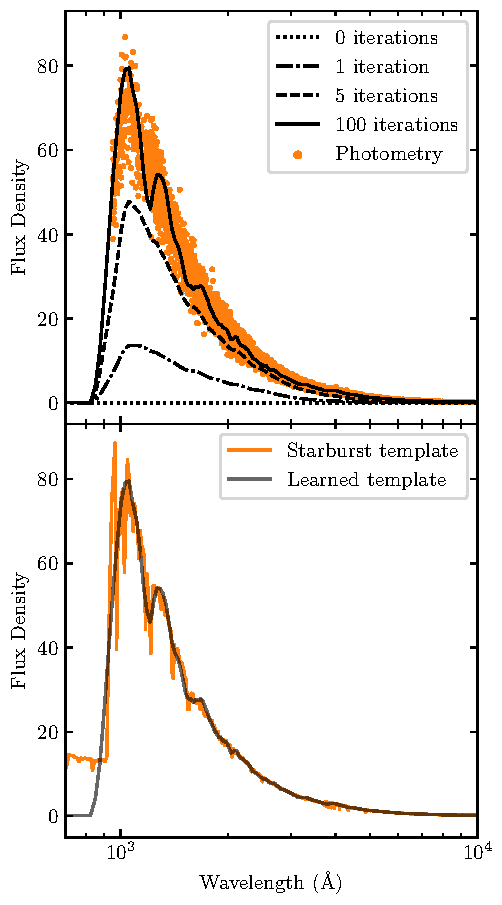
\includegraphics{figures/training_example.pdf}
    \caption{Perturbing a naive template, in this case a flat line, to better match a photometry set. Top: the orange points are simulated observations of the 5Myr starburst template from \citet{Coe2006a} at 1,000 random redshifts in the range z=0 to z=3 using the $ugrizY$ filters listed in Table \ref{tab:filters}. The simulated photometry has 10\% Gaussian error. The template is shown after various stages of the training. Bottom: the learned template is plotted with the original starburst template.}
    \label{fig:pert_ex}
\end{figure}

Iterating the perturbation changes the shape of the template SED to better match the measured photometry, as shown in \citet{Budavari2000b}. 
An example of this process can be seen in Figure \ref{fig:pert_ex}. 
Fluxes in the $ugrizY$ filters listed in Table \ref{tab:filters} were calculated for a starburst galaxy template at 1000 random redshifts $z < 3$. 
Starting with an $S(\lambda) = 0$ template SED, the perturbation algorithm is applied iteratively. 
After 100 iterations, the trained template closely matches the original template in the wavelength range for which photometry exists. 
While the trained template is a smoothed version of the original, high resolution features have been recovered, despite the relatively low resolution of the filters. 
In practice, higher $\Delta_k$ can be chosen so that fewer iterations are required in the training; a lower value was chosen here so that the effects of successive iterations can be more clearly seen.
See Section \ref{sect:hyperparameters} for further discussion of selecting the hyperparameters.

The perturbation algorithm changes the shape of the template SED's so that re-running the photometry matching will now result in different subsets of galaxies assigned to each template.
The full training algorithm is iterated until the SED templates converge.




\subsection{Selecting Hyperparameters}
\label{sect:hyperparameters}

The success of the training algorithm depends on the chosen hyperparameters.
The first is the number of templates. 
As discussed in Section \ref{sect:training_sets}, this choice can be made by using the photometry matching algorithm and choosing the appropriate number of templates to approximately separate out the different spectral shapes displayed in the photometry.
For further discussion of how the number of templates affects photo-z results, see Section \ref{sect:photoz_results}.

The rest of the hyperparameters consist of the set of $\Delta_k$.
These parameters, which set the relative weighting of the regularization term in Equation \ref{eq:cost_function}, determine the stability and speed of the training algorithm.
If the $\Delta_k$ are too large, training will be very slow and a large number of iterations will be required. 
If the $\Delta_k$ are too low, the training becomes unstable and the final templates will be over-fit.
Here we present a heuristic for selecting an appropriate value to balance these two extremes.

For the work presented below, the index $k$ is dropped, so that $\Delta \equiv \Delta_k$ has a single value for each training set that is independent of wavelength. 
In choosing the appropriate value of $\Delta$ for each training set, it is desirable to select a value that corresponds to a constant ratio, $w$, of the flux and regularization terms in Equation \ref{eq:cost_function}. 
The necessary value of $\Delta$ will vary by training set, as the number of terms in the sum over fluxes (i.e. the sum over $n$ in Equation \ref{eq:cost_function}) will vary by training set. 
To this end, we make the following approximation:
\begin{align}
    \frac{\sum_k \left(\hat{s}_k - s_k \right)^2}{\sum_n \left(\hat{f}_n - f_n \right)^2} \sim \frac{N_k}{N_n},
\end{align}
where $N_k \equiv \sum_k$ and $N_n \equiv \sum_n$. 
This permits the following approximation of the ratio $w$: 
\begin{align}
    w = \frac{\sum_k \frac{1}{\Delta^2} \left(\hat{s}_k - s_k \right)^2}{\sum_n \frac{1}{\sigma_n^2} \left(\hat{f}_n - f_n \right)^2} \sim \frac{N_k/\Delta^2}{N_n/\Bar{\sigma}^2},
\end{align}
where $\Bar{\sigma} = \sum_n \sigma_n/N_n$. 
Then, for a desired ratio $w$, the requisite $\Delta$ can be approximated:
\begin{align}
    \Delta \simeq \Bar{\sigma} \sqrt{\frac{N_k}{w N_n}}.
\end{align}
In practice, we have found that $w = \mathcal{O}(1)$ works well.
The results of the training are relatively robust to the selection of $w$, in that changing $w$ by, for example, a factor of 2 yields similar results.
        
\section{Data}
    
\label{sect:data}

We collect a set of galaxy spectroscopic redshifts, paired with broadband photometry, from various surveys to test our training algorithm.
Our set consists of 102,476 galaxies with redshifts $z < 4.54$ and $i$-band magnitudes\footnote{The $i$-band magnitudes quoted in this section denote the magnitude in one of $i$, $i_2$, $I$, or $i^+$ as listed in Table \ref{tab:filters}. For galaxies with photometry in multiple $i$-bands, the magnitude used is the first to appear in that list.} in the range $13.8 < i < 25.7$.
For all surveys, we use galaxies with highly reliable spec-z's, photometry in one of the $i$-bands, and photometry in at least three bands with signal-to-noise ratio SNR $> 20$.
The entire data set is summarized in Table \ref{tab:data_sets}, the filters used to measure the photometry are listed in Table \ref{tab:filters}, and the redshift distributions are shown in Figure \ref{fig:redshift_dist}.

\begin{table*}
    \caption{Summary of the spec-z and photometry data sets. $N_\text{gal}$ is the total number of galaxies in the set, $f_\text{gal}$ is the fraction of galaxies in the set, and $\Bar{\sigma}_i$ is the mean fractional flux error for the $i$-band photometry.}
    \label{tab:data_sets}
    \centering
    \begin{tabular}{l r c c c c c c l}
        \hline \hline
        Data Set & $N_\text{gal}$ & $f_\text{gal}$ & $z_\text{mean}$ & $z_\text{max}$ & $i$-band range & $i_\text{mean}$ & $\Bar{\sigma}_i$ & Link to Catalog \\
        \hline
        
        zCOSMOS  &  14298 & 0.14 & 0.57 & 2.52 & $16.87 \leq i \leq 24.18$ & 21.19 & 0.022 & \url{http://cesam.lam.fr/hstcosmos/} \\
        VVDS     &   6915 & 0.07 & 0.67 & 4.54 & $13.84 \leq i \leq 24.97$ & 20.86 & 0.014 & \url{https://cesam.lam.fr/vvds/index.php} \\
        VIPERS   &  69415 & 0.68 & 0.70 & 2.15 & $17.66 \leq i \leq 23.08$ & 21.38 & 0.017 & \url{http://vipers.inaf.it:8080/} \\
        DEEP2/3  &  10695 & 0.10 & 0.71 & 1.91 & $15.30 \leq i \leq 25.36$ & 21.42 & 0.020 & \url{http://d-scholarship.pitt.edu/36064/} \\
        3D-HST   &   1153 & 0.01 & 1.46 & 3.32 & $19.10 \leq i \leq 25.74$ & 23.56 & 0.027 & \url{http://d-scholarship.pitt.edu/36064/} \\
        \hline
        Training &  81980 & 0.80 & 0.69 & 4.54 & $13.84 \leq i \leq 25.74$ & 21.32 & 0.018 & \\
        Test     &  20496 & 0.20 & 0.69 & 3.61 & $16.46 \leq i \leq 25.69$ & 21.34 & 0.018 & \\
        \hline
        Total    & 102476 & 1.00 & 0.69 & 4.54 & $13.84 \leq i \leq 25.74$ & 21.33 & 0.018 & \\
        
        \hline
    \end{tabular}
\end{table*}

\begin{table}
    \centering
    \caption{The 19 filters used to measure the galaxy photometry in the data set. Mean wavelength, $\lambda_0 = \int \lambda R(\lambda) d\lambda$, and effective width, $W_\text{eff} = \text{Max}[R(\lambda)]^{-1}$, are given in angstroms. Filters are listed in order of increasing $\lambda_0$. The $i_2$ band is the replacement to the Megacam $i$-band installed in 2007. This filter is named $y$ in the CFHTLS catalogues \citep{Hudelot2012}, but we follow \citet{Zhou2019a} in naming it $i_2$ to avoid confusion with the longer $y$ bands used in Subaru and LSST. The system response functions for each filter were obtained from the Spanish Virtual Observatory (SVO) Filter Profile Service.}
    \begin{tabular}{l c c r r}
        \hline \hline
        Filter & Telescope & Instrument & $\lambda_0$ & $W_\text{eff}$ \\
        \hline
        
        $NUV$ & GALEX  &         &  2343.1 &  767.3 \\
        $u$   & CFHT   & Megacam &  3817.7 &  525.4 \\
        $B$   & CFHT   & CFH12k  &  4342.5 &  873.6 \\
        $B_J$ & Subaru & Suprime &  4478.4 &  763.9 \\
        $g^+$ & Subaru & Suprime &  4808.5 & 1043.1 \\
        $g$   & CHFT   & Megacam &  4899.9 & 1293.8 \\
        $V$   & CFHT   & CFH12k  &  5393.7 &  882.7 \\
        $V_J$ & Subaru & Suprime &  5493.0 &  862.4 \\
        $r$   & CHFT   & Megacam &  6278.2 & 1120.2 \\
        $r^+$ & Subaru & Suprime &  6314.8 & 1211.4 \\
        $R$   & CFHT   & CFH12k  &  6603.5 & 1138.5 \\
        $i_2$ & CHFT   & Megacam &  7584.5 & 1409.4 \\
        $i$   & CHFT   & Megacam &  7676.6 & 1307.6 \\
        $i^+$ & Subaru & Suprime &  7709.1 & 1361.7 \\
        $I$   & CFHT   & CFH12k  &  8277.3 & 1816.7 \\
        $z$   & CHFT   & Megacam &  8857.6 & 1040.1 \\
        $z^+$ & Subaru & Suprime &  9054.5 & 1012.3 \\
        $Y$   & Subaru & Suprime & 10216.0 &  996.2 \\
        $J$   & UKIRT  & WFCAM   & 12508.5 & 1476.8 \\
        
        \hline
    \end{tabular}
    \label{tab:filters}
\end{table}

\subsection{zCOSMOS-\textit{bright}}

zCOSMOS \citep{Lilly2009a} is a redshift survey of 1.7 $\text{deg}^2$ of the COSMOS field, conducted with the VIMOS spectrograph mounted on the European Southern Observatory's (ESO) Very Large Telescope (VLT).
The survey is divided into two parts, \textit{bright} and \textit{deep}. 
We make use of the former, consisting of approximately 20,000 galaxies with redshifts $z < 1.2$.
We use galaxies recommended in the ESO data release description\footnote{\url{https://www.eso.org/sci/observing/phase3/data_releases/zcosmos_dr3_b2.pdf}}, determined to have $99\%$ spectroscopic verification (i.e. \texttt{zflag} = 3.x, 4.x, 2.5, 2.4, 1.5, 9.5, 9.3, 18.5, 18.3).

The zCOSMOS redshifts are matched to photometry from \citet{Ilbert2009}.
The photometry is measured from the ultraviolent to the near-infrared in 11 broadband filters: $NUV$ on GALEX \citep{Martin2005a}, $u$ and $i$ on CFHT-Megacam, $B$ and $V$ on CFHT-CFH12k, $g^+$, $r^+$, $i^+$, and $z^+$ on Subaru, and $J$ on UKIRT.
We use only galaxies detected in all of the optical bands.
The final set consists of 14,298 galaxies with redshifts $z < 2.52$ and $i$-band magnitudes in the range $16.9 < i < 24.2$.

\subsection{VVDS}

The VIMOS VLT Deep Survey (VVDS, \citealt{LeFevre2013b}) is a redshift survey consisting of three component surveys: \textit{Wide}, \textit{Deep}, and \textit{Ultra-Deep}. 
The Wide survey covers 8.7 $\text{deg}^2$, with approximately 25,000 galaxies in the range $17.5 < i < 22.5$; the Deep survey covers 0.74 $\text{deg}^2$, with approximately 11,000 galaxies in the range $17.5 < i < 24$; the Ultra-Deep survey covers 512 $\text{arcmin}^2$, with approximately 900 galaxies in the range $23 < i < 24.75$.
We use redshifts with quality flags 3 and 4, indicating a 98\% spec-z confidence.
The photometry was measured in nine filters: $u,g,r,i,z$ on CFHT-Megacam \citep{Hudelot2012} and $B,V,R,I$ on CFHT-CFH12k \citep{LeFevre2004}.
The final set contains 6,915 galaxies out to redshifts $z < 4.5$, with magnitudes $ 13.8 < i < 25.0$.

\subsection{VIPERS}

The VIMOS Public Extragalactic Redshift Survey (VIPERS, \citealt{Scodeggio2018a}) is a dense, large-volume redshift survey focusing on redshifts $0.5 < z < 1.2$.
We use VIPERS galaxies with spec-z's reliable at the 95\% confidence level (\texttt{zflag} = 2.X, 3.X, 4.X), and with \texttt{photoMask} and \texttt{spectroMask} = 1.
The redshifts are matched to photometry measured in $NUV$ on GALEX \citep{Martin2005a}, and $u,g,r,i_2,i,z$ on CFHT-Megacam \citep{Hudelot2012}. 
The final set contains 71,951 galaxies with redshifts $z < 2.15$ and magnitudes $17.7 < i < 23.3$. 

\subsection{DEEP2 and DEEP3}

DEEP2 and DEEP3 are redshift surveys conducted with the DEIMOS spectrograph on the Keck 2 telescope.
DEEP2 \citep{Newman2013b} consists of four fields; we use galaxies from the first field in the Extended Groth Strip (EGS), which had no redshift pre-selection.
DEEP3 \citep{Cooper2011} expanded on the DEEP2 survey of the EGS.
Redshifts from these surveys are matched with aperture-corrected photometry provided by \citet{Zhou2019a}.
We use galaxies with CFHTLS flag 0, SExtractor flags less than 4 in every band, and redshift quality flag $\geq 3$.
Photometry was measured in $u,g,r,i_2,i,z$ on CFHT-Megacam and $Y$ on Subaru \citep{Miyazaki2002}.
The final set contains 10,695 galaxies with redshifts $z < 1.91$ and magnitudes $15.3 < i < 25.74$.


\subsection{3D-HST}

In addition to the spectroscopic surveys above, we include grism redshifts from the 3D-HST survey \citep{Newman2013b,Momcheva2016b}.
Redshifts for this survey were analyzed and matched with aperature-corrected photometry by \citet{Zhou2019a}.
We select the galaxies with CFHTLS flag 0, SExtractor flags less than 4 in every band, and the flag \texttt{use\_zgrism1} = 1.
For galaxies in both the DEEP2/3 and 3D-HST sets, we use DEEP2/3 redshifts instead.
Photometry was measured in $u,g,r,i_2,i,z$ on CFHT-Megacam and $Y$ on Subaru.
After these cuts, the 3D-HST set contains 1,153 galaxies with redshifts $z < 3.32$ and magnitudes $23.6 < i < 25.7$.


\begin{figure}
    \centering
    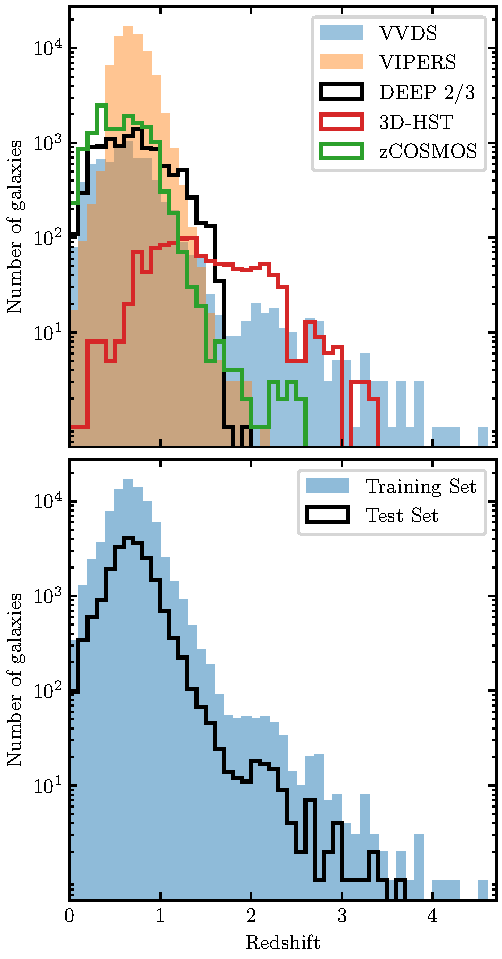
\includegraphics{figures/redshift_distribution.pdf}
    \caption{Redshift distribution of the galaxy surveys. The top panel shows the distributions of each of the constituent surveys. The bottom panel shows the redshift distributions of the training and test sets used for template training and photo-z estimation respectively.}
    \label{fig:redshift_dist}
\end{figure}



\section{Application to Data}
    
\label{sect:application}

\note{Start by describing the training and test sets here.
Mention their redshift and magnitude ranges.
Calculate the min and max wavelength of the training set, and say that we will try to reconstruct spectra over that wavelength range.}




\subsection{The Training and Test Set}

\note{Move discussion of the training and test set here.}




\subsection{Training Templates on the Data}

Eight naive templates were chosen to represent the underlying SED shapes of the data set according to the principles described at the end of Section \ref{sect:training_sets}. 
They are ``naive'' because they are just chosen by eye to roughly split the photometry into groups by shape. 
Each is a log-normal distribution,
\begin{align}
    S(\lambda) \propto \frac{1}{\lambda} \exp{\left[ -\frac{1}{2\sigma^2} \left( \ln{\frac{\lambda}{\text{mode}(\lambda)}}-\sigma^2 \right)^2 \right]},
\end{align}
normalized at $\lambda = 5000$ \AA, with $\text{mode}(\lambda)$ in the range $1000$ to $5500$ \AA\  and $\sigma$ in the range $0.35$ to $0.9$. 
\note{100 \AA\ tophat bins.}
These eight templates (hereafter N8) can be seen together with with their original training sets in Figure \ref{fig:N8_untrained}.

\begin{figure*}
    \centering
    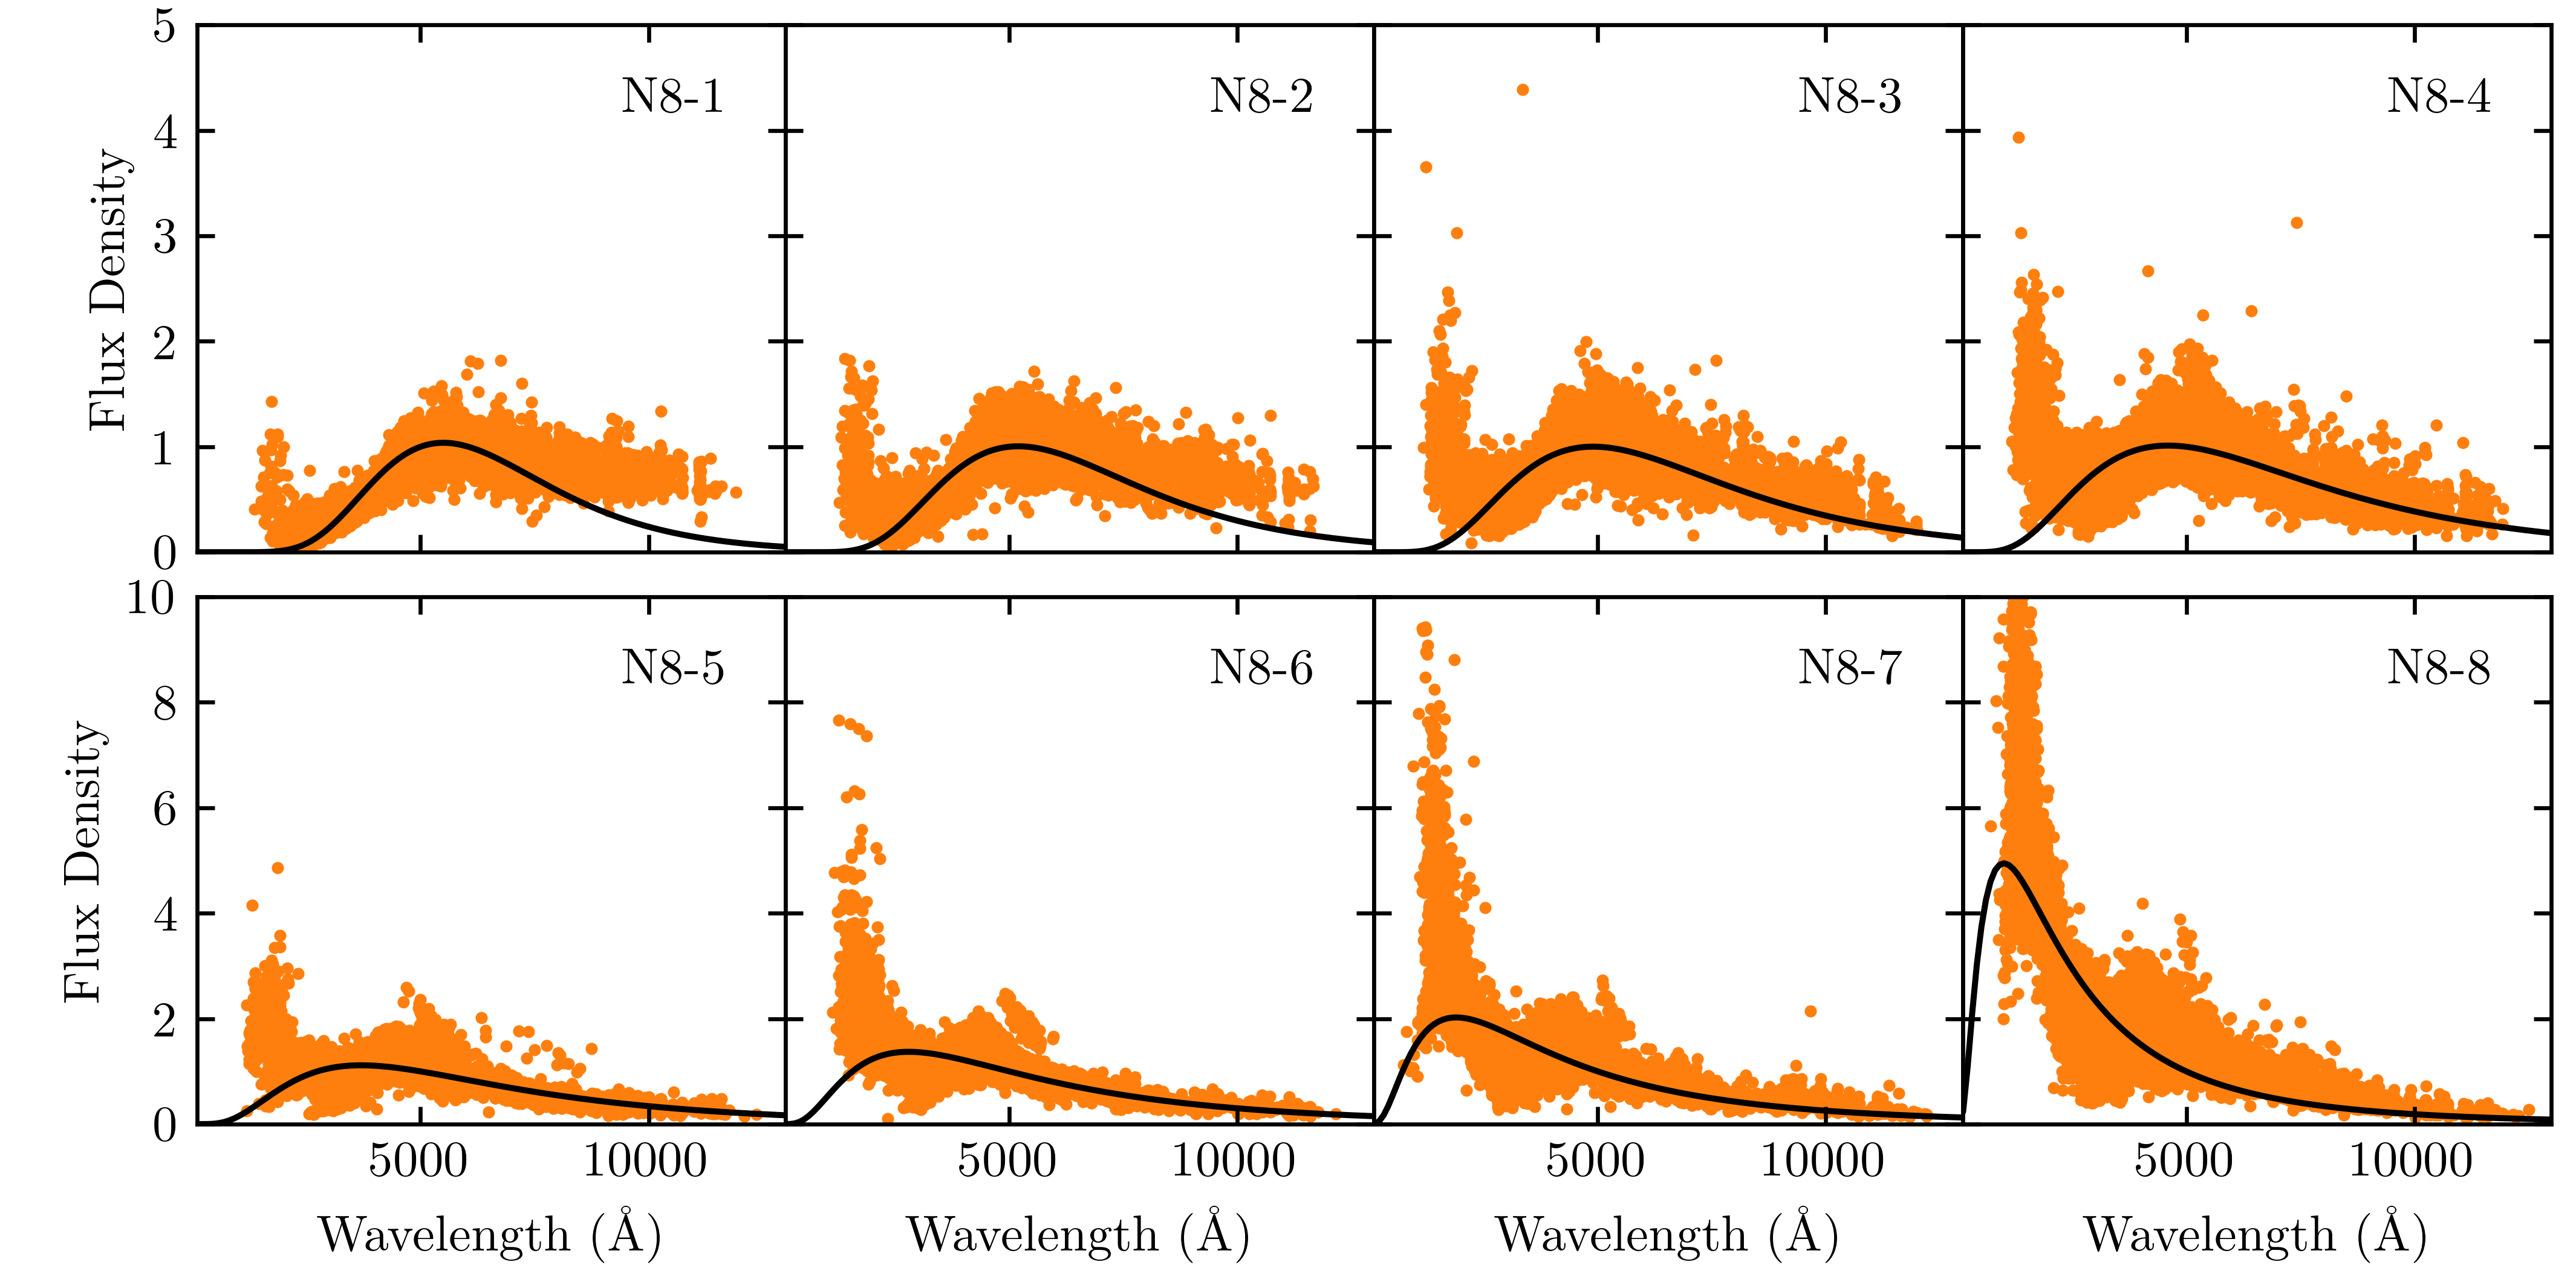
\includegraphics{figures/N8_untrained.png}
    \caption{The untrained N8 templates (black lines) with their original training sets (orange points). N8 1 is the reddest template, with each successive template getting bluer.}
    \label{fig:N8_untrained}
\end{figure*}

These eight templates were chosen to approximately separate the galaxy photometry into distinct groups based on spectral shape, and to ensure that each template had a sizeable and well distributed training set. 
While this requires some guess and check with the assembled training sets, the strength of this method is that you do not need a priori information of galaxy spectra.

After the training sets are assembled, outliers are removed by means of an Isolation Forest in the flux-wavelength space. 
Outliers are determined on a per-flux basis instead of per-galaxy. 
Removing outliers before training the templates helps stabilize the results of the perturbation algorithm described in the next section.

The training algorithm is applied to the N8 templates, resulting in the final templates seen in Figure \ref{fig:N8_trained}. 
The templates were trained for five rounds, with each round consisting of three perturbations with $w=0.5$. 
After the training, the templates more closely resemble real galaxy spectra. 
You can see there are now features in the templates at a much higher resolution than the broadband filters. 
\note{Add lines to guide the eye for 400nm break and spectral lines, where they are visible. Mention those here as well.}

\begin{figure*}
    \centering
    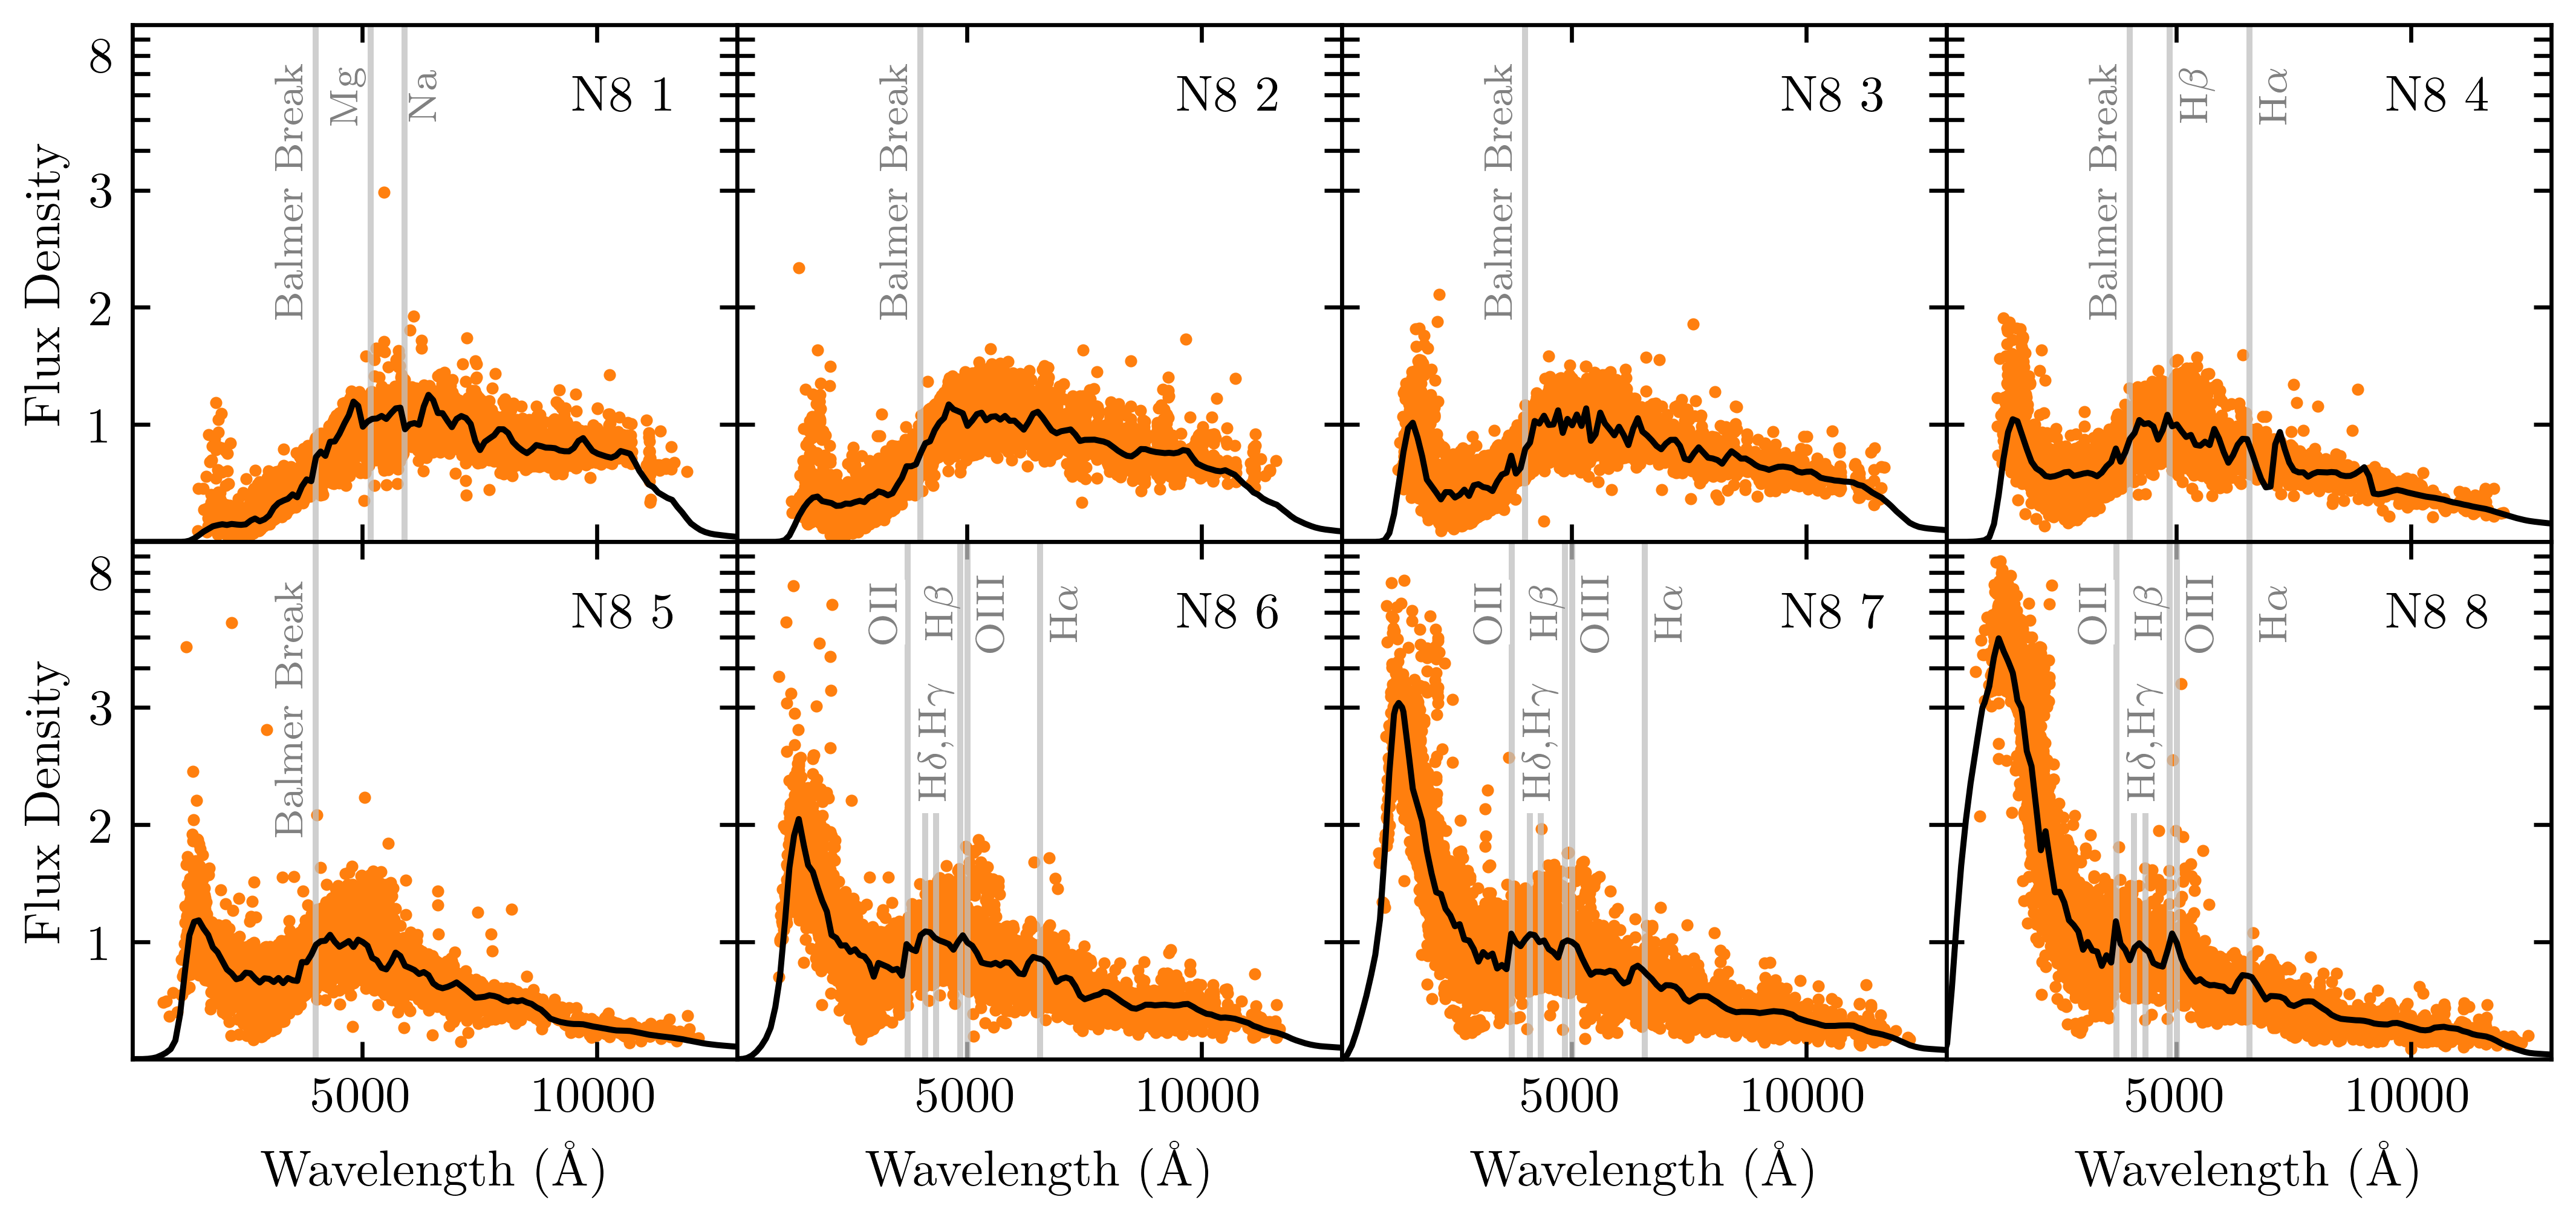
\includegraphics{figures/N8_trained.png}
    \caption{The trained N8 templates (black lines) with their final training sets (orange points). N8 1 is the reddest template, with each successive template getting bluer. \note{Say something about the lines added to guide the eye to spectral features.}}
    \label{fig:N8_trained}
\end{figure*}

In addition to these eight templates, we also train a set of 16 templates from the same range of parameters for the log-normal distribution, creating a more gradual transition of the templates from red to blue. 
This template set (hereafter N16) can be seen with the final training sets in Figure \ref{fig:N16_trained}. 
These were again trained for five rounds, with each round consisting of three perturbations with $w=0.5$. 

\begin{figure*}
    \centering
    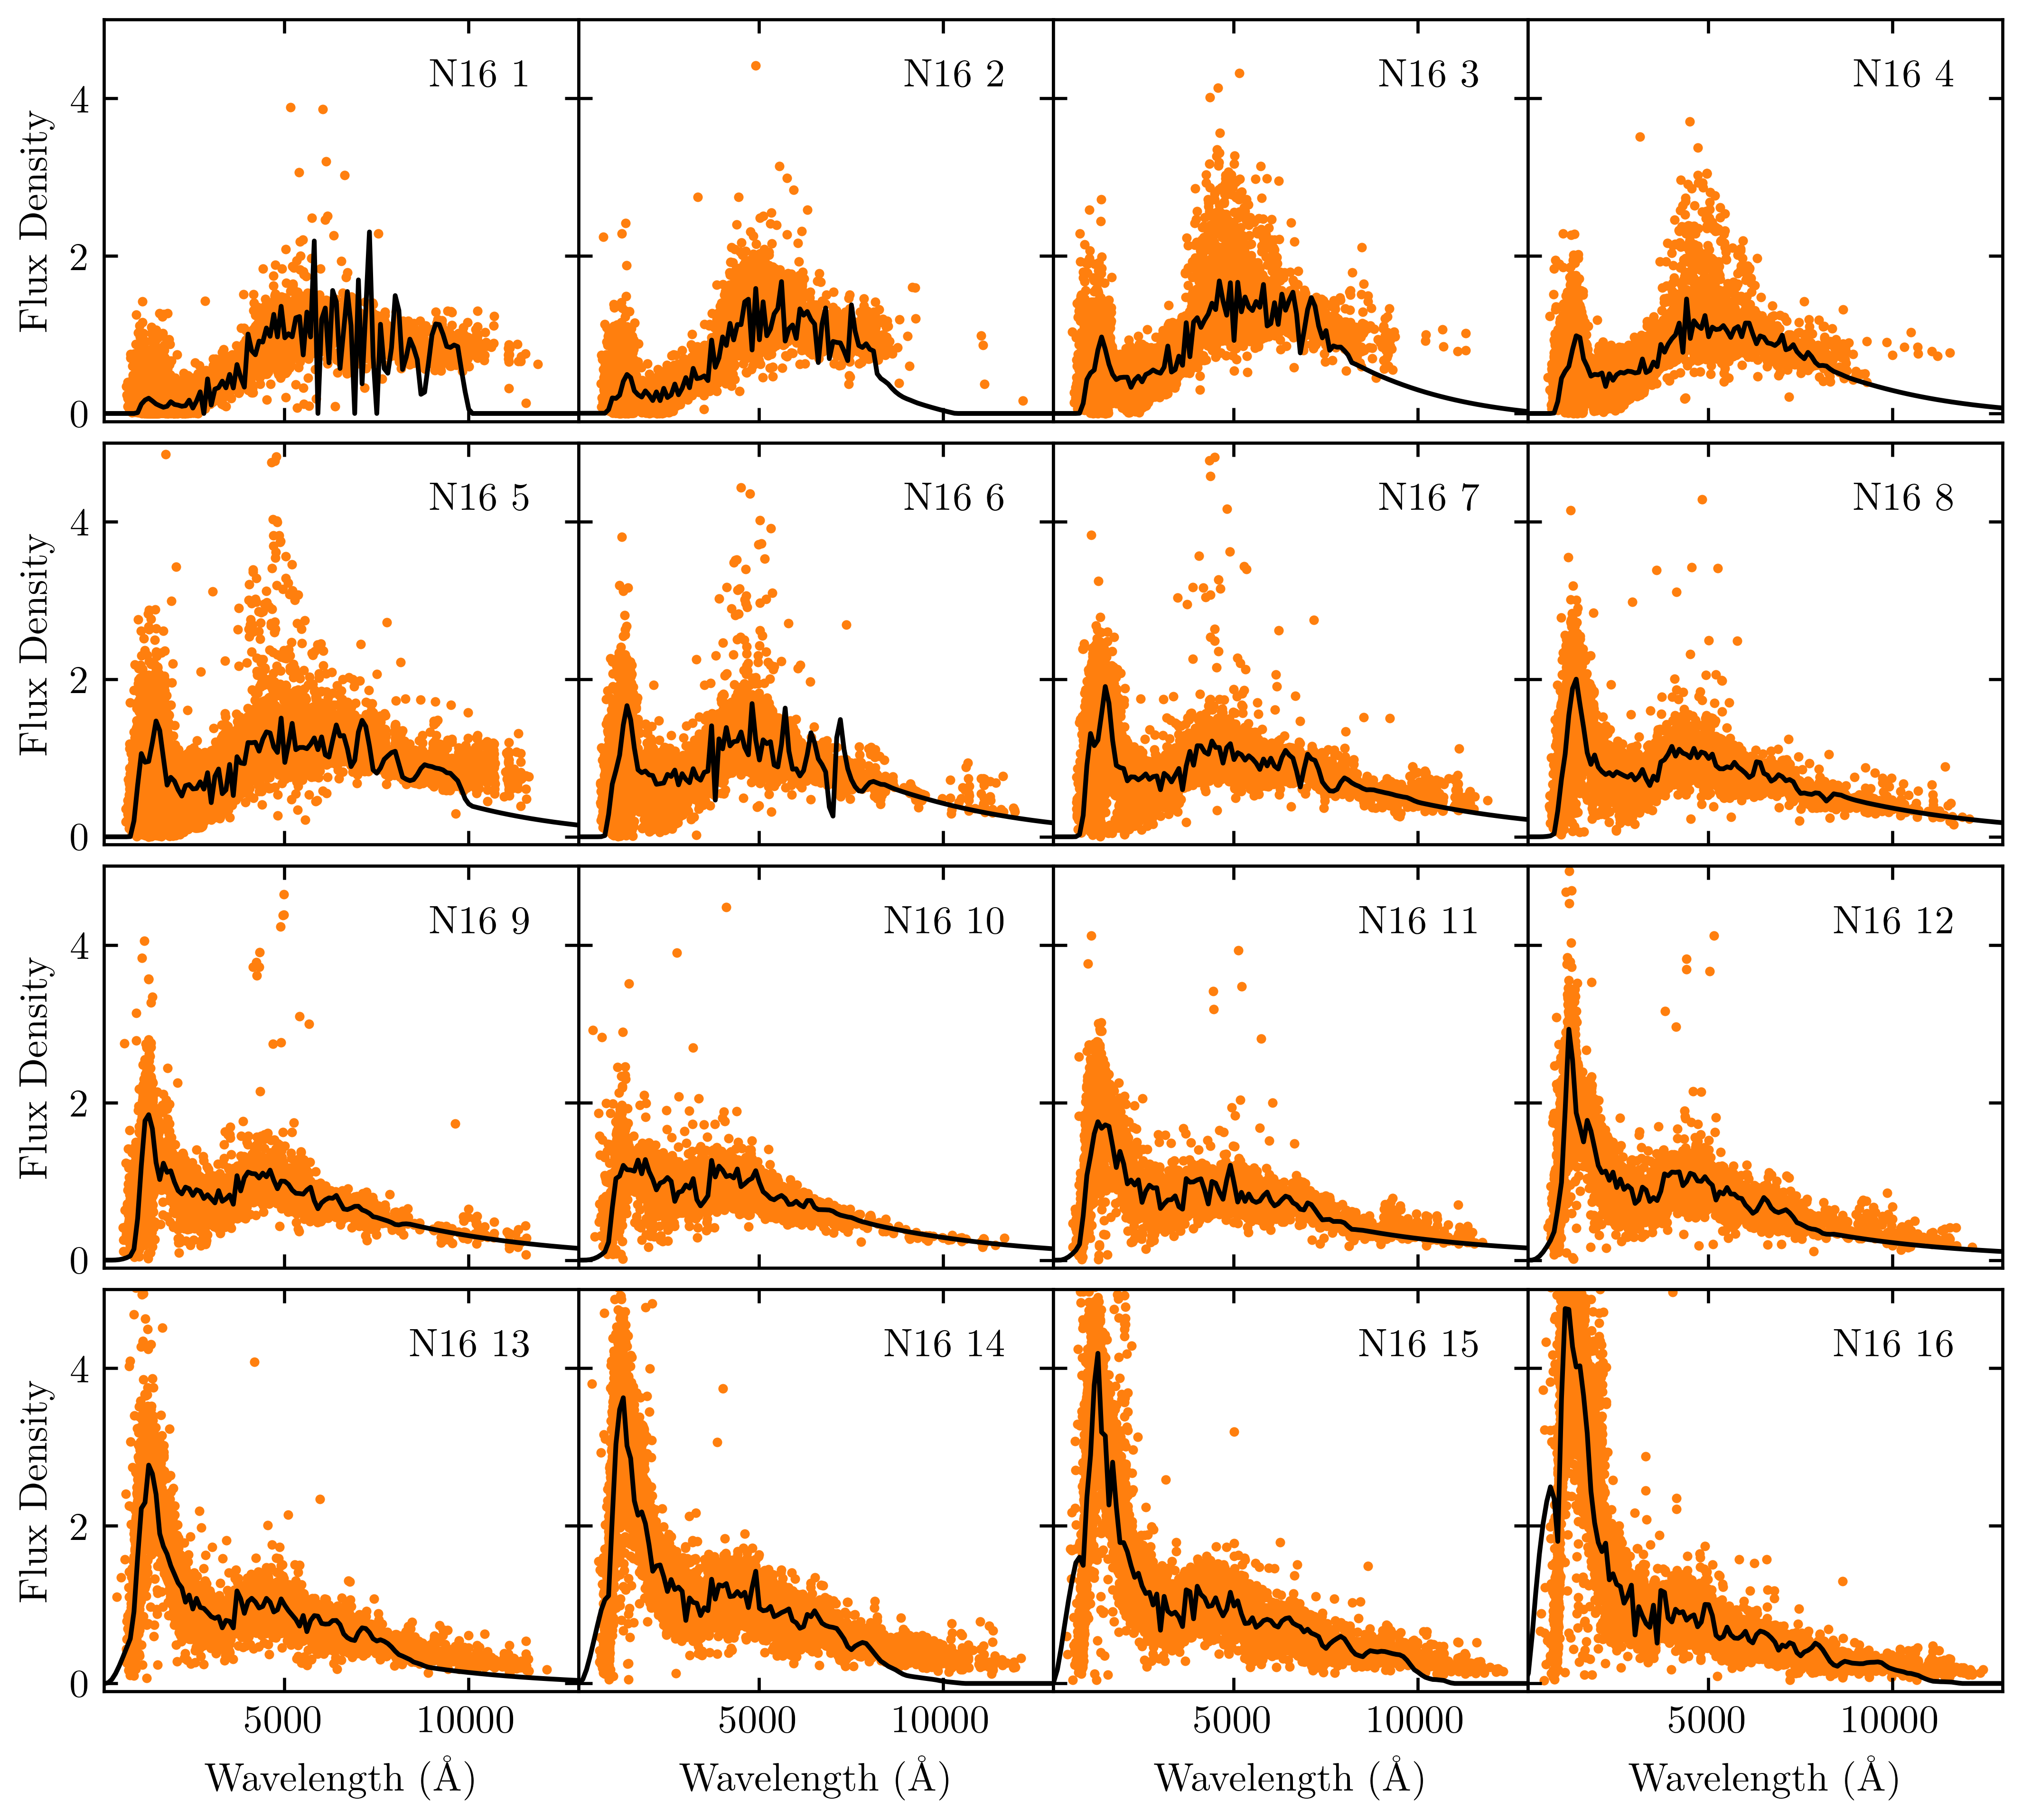
\includegraphics{figures/N16_trained.png}
    \caption{The trained N16 templates (black lines) with their final training sets (orange points). N16 1 is the reddest template, with each successive template getting bluer. \note{Say something about the lines added to guide the eye to spectral features.}}
    \label{fig:N16_trained}
\end{figure*}

In addition to starting from naive templates, one can start with templates derived from spectral synthesis models or observations of local galaxy spectra. 
Here we apply the training algorithm to a standard set of SED templates that comes with \bpz.
This set (hereafter CWW+SB4) consists of four templates from \citet{Coleman1980a} and two starburst templates from \citet{Kinney1996a}, the latter of which were added to account for faint blue galaxies in the HDF-N. 
These six templates were recalibrated by \citet{Benitez2004a} to correct for systematic differences between the observed and predicted galaxy colors in the HDF-N and other spectroscopic catalogs. 
In addition to these six, CWW+SB4 contains two synthetic starburst templates from \citet{Bruzual2003b}, added by \citet{Coe2006a} to account for even bluer galaxies in the UDF.

These templates were trained for five rounds, with each round consisting of one perturbation with $w=2$. 
The results of the training can be seen together with the original CWW+SB4 templates and the final training sets in Figure \ref{fig:cwwsb4_trained}. 
\note{Say something about how the training added additional high resolution structure to the templates and added a red tilt to Im, SB2, 25Myr, and 5Myr.}

\begin{figure*}
    \centering
    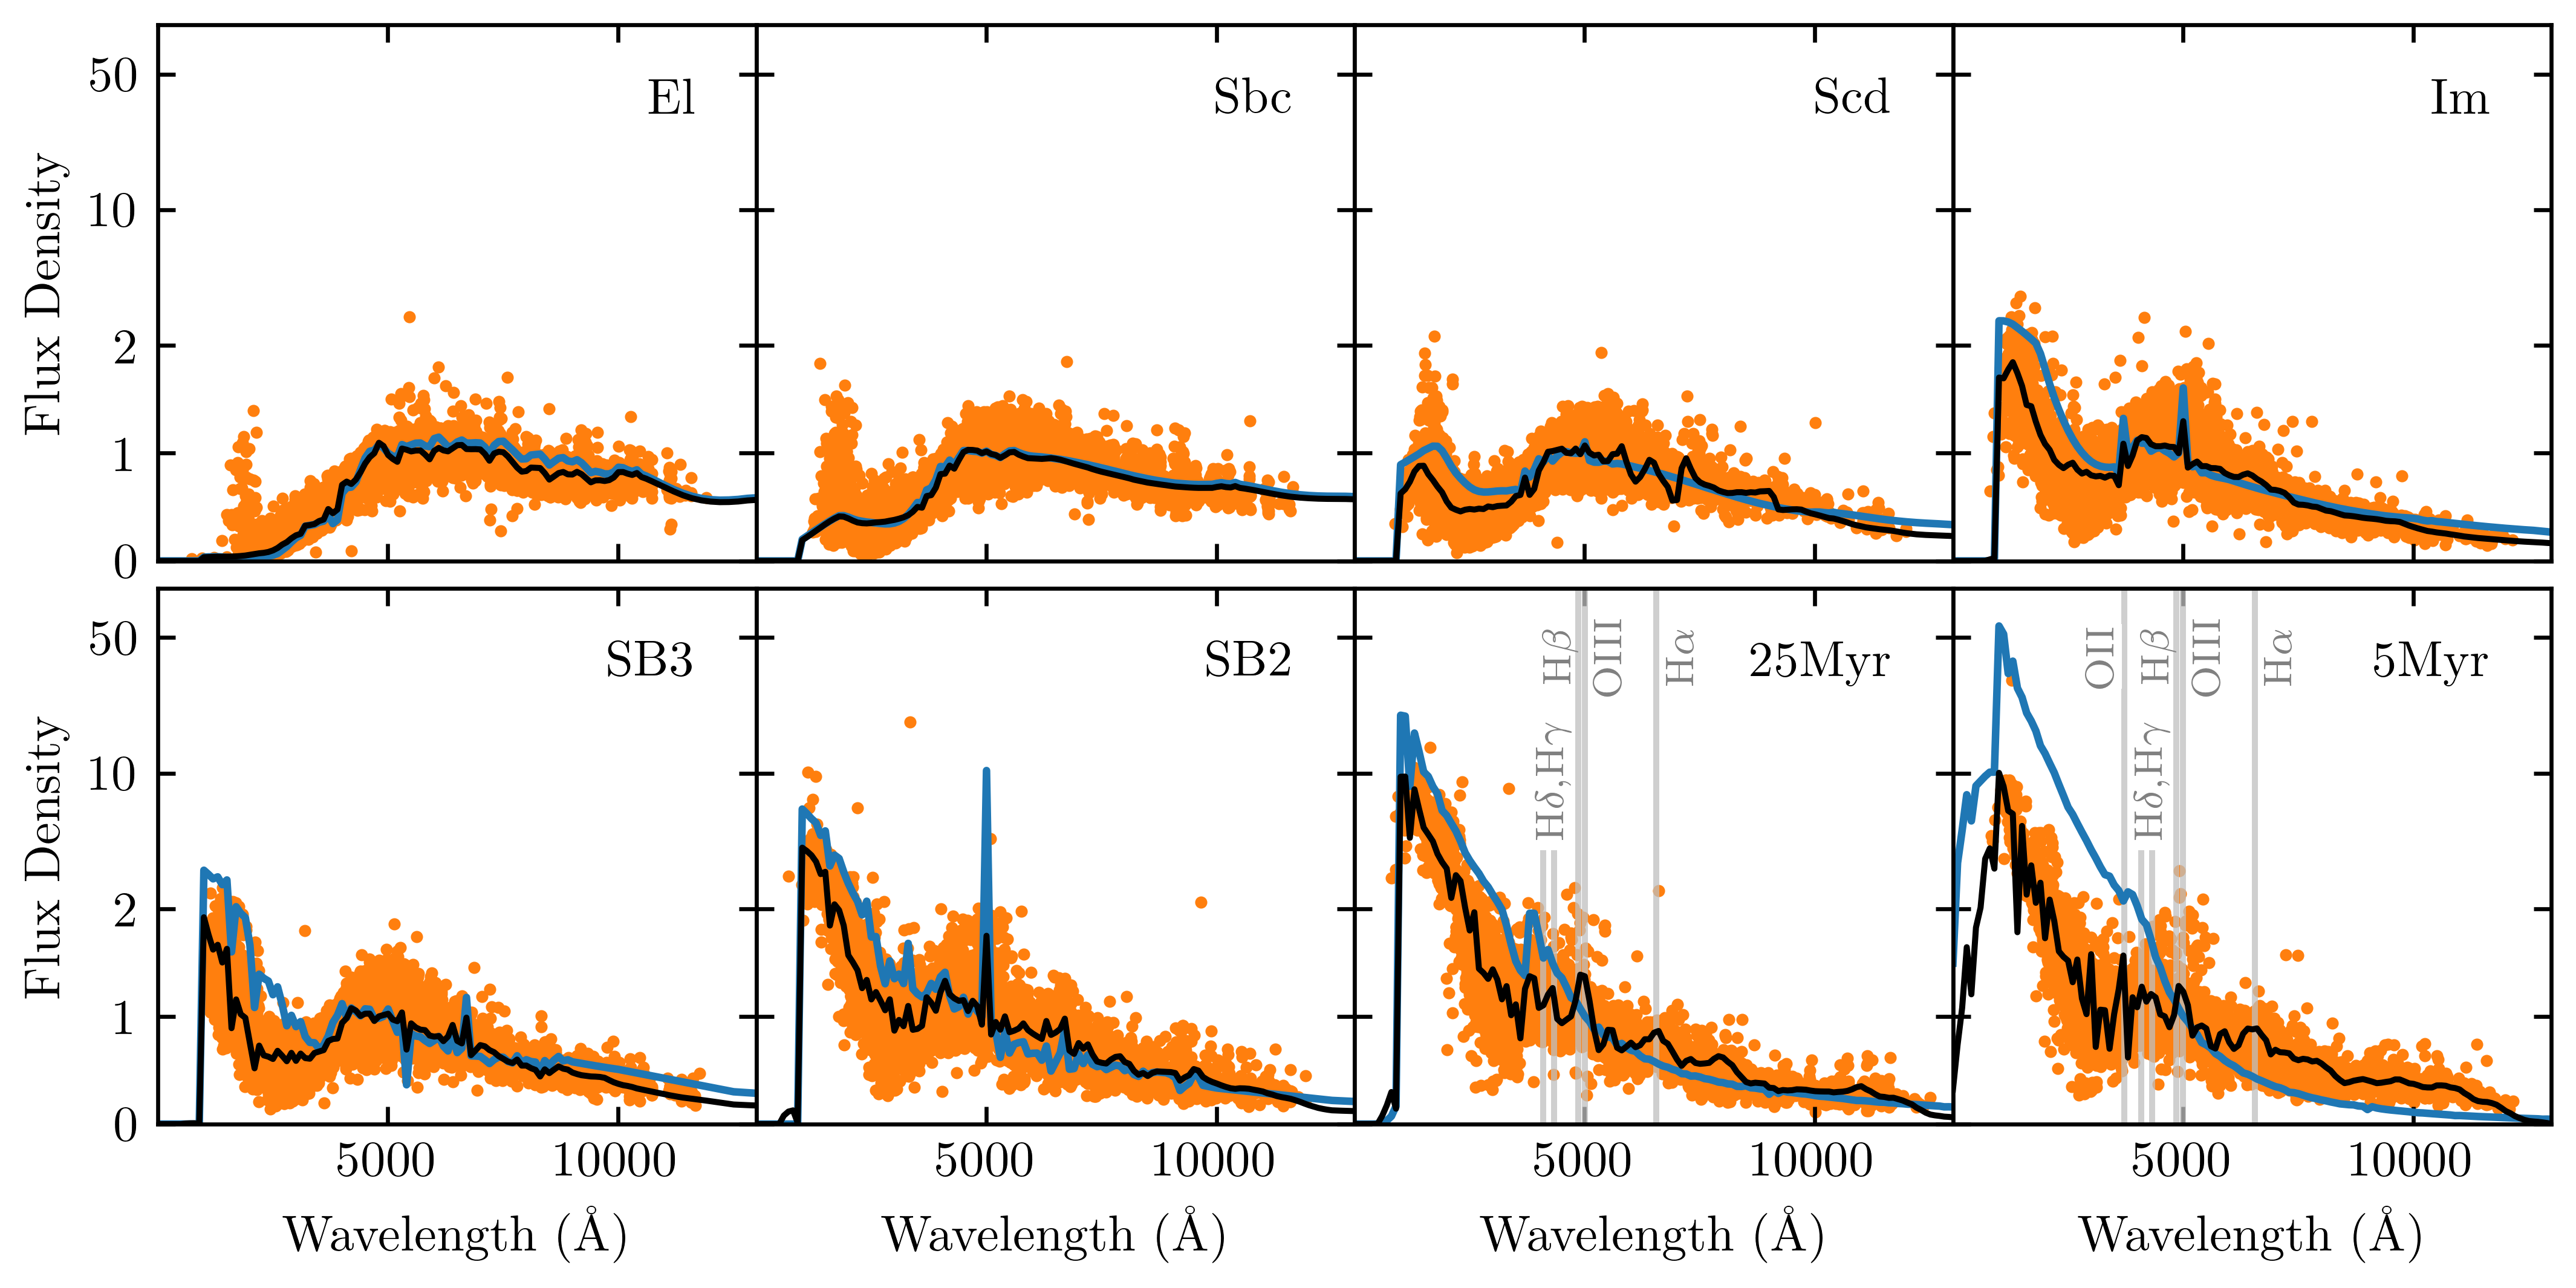
\includegraphics{figures/cwwsb4_trained.png}
    \caption{Result of training the CWW+SB4 templates. The original templates are in blue, the trained templates in black, and the final training sets are displayed as orange points.}
    \label{fig:cwwsb4_trained}
\end{figure*}

% here's a good link for spectral lines
% http://star-www.st-and.ac.uk/~spd3/Teaching/PHYS1002/phys1002_lecture6.pdf
% and here's the spectral ratios
% https://arxiv.org/pdf/1109.2597.pdf  
    
\section{Estimating Photo-z's}
    
\label{sect:photoz}

We evaluate the results of our template training algorithm by using our learned templates to estimate photo-z's for the test set of galaxies using the software package \bpz\ \citep{Benitez2000a}, and comparing the results to the spec-z's and the photo-z's estimated using the original CWW+SB4 templates.
The test set consists of 20,496 galaxies (20\% of the total set), with mean redshift $z_\text{mean} = 0.69$, max redshift $z_\text{max} = 3.61$, and magnitudes $13.8 < i < 25.7$.
See Table \ref{tab:data_sets} for a full summary and Figure \ref{fig:redshift_dist} for the redshift distribution.

\subsection{Bayesian Photometric Redshifts}
\label{sect:bpz}

Bayesian Photometric Redshifts (\bpz; \citealt{Benitez2000a}) is a template-based photo-z estimator.
Template-based estimators take a set of SED templates, assumed to be spanning and exclusive, and calculate observed fluxes over a grid of redshift values. 
Each set of observed fluxes is then matched to a specific template and redshift determined to be the most likely to have produced the observed colors. 

For each template, \bpz\ evaluates a $\chi^2$ function at each redshift on the grid:
\begin{align}
    \chi^2 (z,T,A) = \sum_n \frac{1}{\sigma_n^2} (\, A \, \hat{f}_n(z,T) - f_n \,)^2,
    \label{eq:chi2}
\end{align}
where $T$ denotes the template, $z$ denotes the redshift, $A$ is a normalization, and $\hat{f}_n$, $f_n$, and $\sigma_n$ denote the calculated flux, the observed flux, and the fractional error as in Equation \ref{eq:cost_function}. 
The sum over $n$ is a sum over the filters for the set of observed fluxes. 
\bpz\ then evaluates the likelihood for producing the observed galaxy fluxes: $p(\{f_n\}|z,T) \propto \exp{(-\chi^2/2)}$. 
The redshift posterior is then calculated by marginalizing over the set of templates:
\begin{align}
    p(z|\{f_n\},m_0) &= \sum_T \, p(z,T|\{f_n\},m_0) \nonumber \\
                     &\propto \sum_T \, p(z,T|m_0) \, p(\{f_n\}|z,T),
\end{align}
where $p(z,T|m_0)$ is a prior over the apparent magnitude $m_0$. 
Work is underway to determine how best to use the full information encoded in the redshift posterior generated by \bpz\ and other photo-z codes (e.g. \citealt{Schmidt2020}). 
In this work, however, only the mode of the posterior distribution is used to estimate the photo-z.

We use \bpz-v1.99.3\footnote{\url{http://www.stsci.edu/~dcoe/BPZ/}} to estimate photo-z's.
We turn off template interpolation by setting \texttt{INTERP=0}.
For simplicity, we treat non-detections as non-observations.
We use the various sets of SED templates described in Section \ref{sect:application}, and use the prior described in the following section.
All other settings were left as default.


\subsection{Galaxy Magnitude Priors}

Before estimating photo-z's with \bpz, we must first construct the magnitude priors, $p(z,T|m_0)$, calibrated to the galaxies in our training set.
We separate the prior into two parts:
\begin{align}
    p(z,T|m_0) = p(T|m_0) \, p(z|T,m_0)
\end{align}
For the magnitude $m_0$, we use one of the $i$ bands in the following order of priority: $i$, $i_2$, $I$, $i^+$.
Instead of constructing a different prior for each template, we follow \citet{Benitez2000a} in dividing our templates into three broad classifications: elliptical (El), spiral (Sp), or irregular/starburst (Im/SB).
The CWW+SB4 templates are already classified under this scheme.
We classify our new templates and each of the galaxies in the training set by assigning the classification of the CWW+SB4 template with the most similar colors, determined by minimizing the mean square error of the fluxes.
The N8 templates are determined to have one elliptical, four spiral, and three irregular/starburst galaxies; the N16 templates are determined to have two elliptical, eight spiral, and six irregular/starburst galaxies.
The fraction of each classification as a function of magnitude for the training set galaxies is displayed in Figure \ref{fig:class_vs_mag}.

We assume that the El and Im/SB galaxies have spectral priors of the form
\begin{align}
    p(T|m_0) = \frac{L_T}{1+e^{-\kappa_T(m_0 - m_T)}} + C_T,
\end{align}
while $p(\text{Sp}|m_0) = 1 - p(\text{El}|m_0) - p(\text{Im/SB}|m_0)$.
The values of $\{L_T,\kappa_T,m_T,C_T\}$ for the El and Im/SB galaxies are found by fitting to the distributions in Figure \ref{fig:class_vs_mag}.
All three priors are plotted in the same figure, and the parameter values are listed in Table \ref{tab:prior_params}.

\begin{figure}
    \centering
    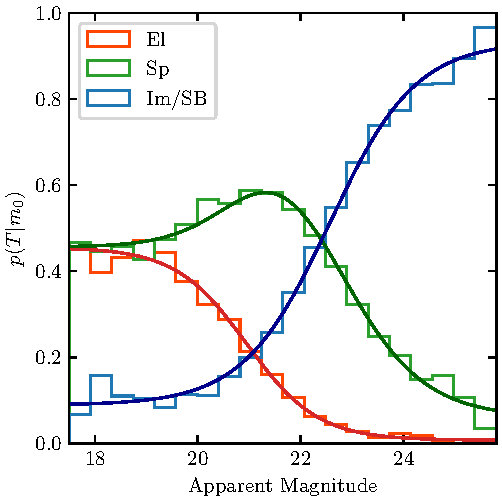
\includegraphics{figures/class_vs_mag.pdf}
    \caption{Fraction of each spectral class as a function of apparent magnitude. The histograms represent the fractions in the training set, and the curves are the spectral type priors fit to the data.}
    \label{fig:class_vs_mag}
\end{figure}

For the redshift prior, we use Equations 23 and 24 from \citet{Benitez2000a}:
\begin{align}
    p(z|T,m_0) = \frac{1}{N_T} \exp \left\{ -\left( \frac{z}{Z_T} \right)^{\alpha_T} \right\},
    \label{eq:z_prior}
\end{align}
where the normalization is
\begin{align}
    N_T = \frac{Z_T^{~\alpha_T + 1}}{\alpha_T} ~ \Gamma \left( \frac{\alpha_T + 1}{\alpha_T} \right),
\end{align}
and the ``median'' redshift $Z_T$ is chosen to have the linear dependence
\begin{align}
    Z_T(m_0) = z_{0T} + k_T(m_0 - 20).
\end{align}
Equation \ref{eq:z_prior} reproduces the exponential cutoff at high redshifts present in the training set, and can reasonably approximate any unimodal redshift distribution, from very narrow ($\alpha \gg 2$) to very broad ($\alpha \ll 1$).
This flexibility reduces the bias introduced by the functional form of the prior \citep{Benitez2000a}.
The nine parameters $\{\alpha_T, z_{0T}, k_T\}$ are determined by maximizing the likelihood $L = \prod_i p(z_i|T_i,m_{0i})$, where the product is over the galaxies in the training set.
The parameters and their bootstrapped uncertainties are listed in Table \ref{tab:prior_params}.

\begin{table*}
    \caption{Parameters for the priors, $p(z,T|m_0)$.}
    \label{tab:prior_params}
    \centering
    \begin{tabular}{l c c c c c c c }
        \hline \hline
         Spectral Type & $L_T$ & $\kappa_T$ & $m_T$ & $C_T$ & $\alpha_T$ & $z_{0T}$ & $k_T$ \\
         \hline
         
         El & $0.448 \pm 0.017$ & $-1.45 \pm 0.16$ & $21.0 \pm 0.1$ & $0.007 \pm 0.009$ & $3.88 \pm 0.04$ & $0.484 \pm 0.003$ & $0.119 \pm 0.002$ \\
         Sp & - & - & - & - & $3.40 \pm 0.04$ & $0.493 \pm 0.003$ & $0.124 \pm 0.002$ \\
         Im/SB & $0.845 \pm 0.031$ & $1.20 \pm 0.11$ & $22.6 \pm 0.1$ & $0.089 \pm 0.013$ & $2.22 \pm 0.03$ & $0.361 \pm 0.009$ & $0.130 \pm 0.008$ \\
        
        \hline
    \end{tabular}
\end{table*}


\subsection{Photo-z Results}
\label{sect:photoz_results}

We estimate photo-z's for the test set galaxies using \bpz\ with the settings and priors described in the previous two sections.
We used four template sets: the original CWW+SB4 templates, the trained CWW+SB4 templates, and the trained N8 and N16 templates.

\bpz\ provides two metrics for the photo-z estimates: \texttt{ODDS} and $\chi_{\text{mod}}^2$.
\texttt{ODDS} measures how narrowly peaked the posterior distribution $p(z|\{f_n\},m_0)$ is around the estimated photo-z.
Galaxies with low \texttt{ODDS} have either broad redshift posteriors, or posteriors with multiple peaks.
$\chi_{\text{mod}}^2$ measures how well the best fit template at the predicted redshift matches the observed fluxes. 
For more about these metrics, see Section 4 of \citet{Benitez2000a} and Section 4.3 of \citet{Coe2006a}.
In this work, photo-z estimates with \texttt{ODDS} $< 0.95$ or $\chi_{\text{mod}}^2 > 1$ are excluded from the analysis, and the fraction excluded on this bases is reported as $f_\text{cut}$.

To further evaluate the results of \bpz, we calculate the scatter, bias, and outlier fraction of the photo-z estimates. 
Photo-z estimates are known to be contaminated with a significant number of outliers.
This is largely driven by a degeneracy wherein the 1000\AA\ Lyman break in a high redshift galaxy spectrum is shifted to the position of the 4000\AA\ Balmer break in a low redshift galaxy spectrum. 
\bpz\ attempts to break this degeneracy with the galaxy magnitude prior (i.e. galaxies with brighter apparent magnitudes are more likely to be at a lower redshift), yet there are still a large number of outliers.

To address this issue, we evaluate the statistics of the interquartile range (IQR) of the data, as these measures are robust to the presence of outliers.
We follow \citet{Graham2018a} in introducing the quantity $\Delta z_{1+z} = (z_{spec} - z_{phot})/(1 + z_{phot})$.
The numerator quantifies the photo-z error and the denominator compensates for the larger uncertainty at high redshifts. 
We define the scatter of the photo-z estimates, $\sigma_\text{IQR}$,  as the width of the IQR in $\Delta z_{1+z}$, divided by 1.349 to convert to the equivalent of a Gaussian standard deviation. 
We define the bias of the photo-z estimates as the mean value of $\Delta z_{1+z}$ for galaxies within the IQR.
The uncertainties of these two values are bootstrapped by calculating the values on 1000 random samples with replacement. 
Outliers are identified as photo-z's with $\Delta z_{1+z} > 3 \sigma_{\text{IQR}}$, and the fraction of outliers is reported as $f_\text{out}$.

\begin{figure*}
    \centering
    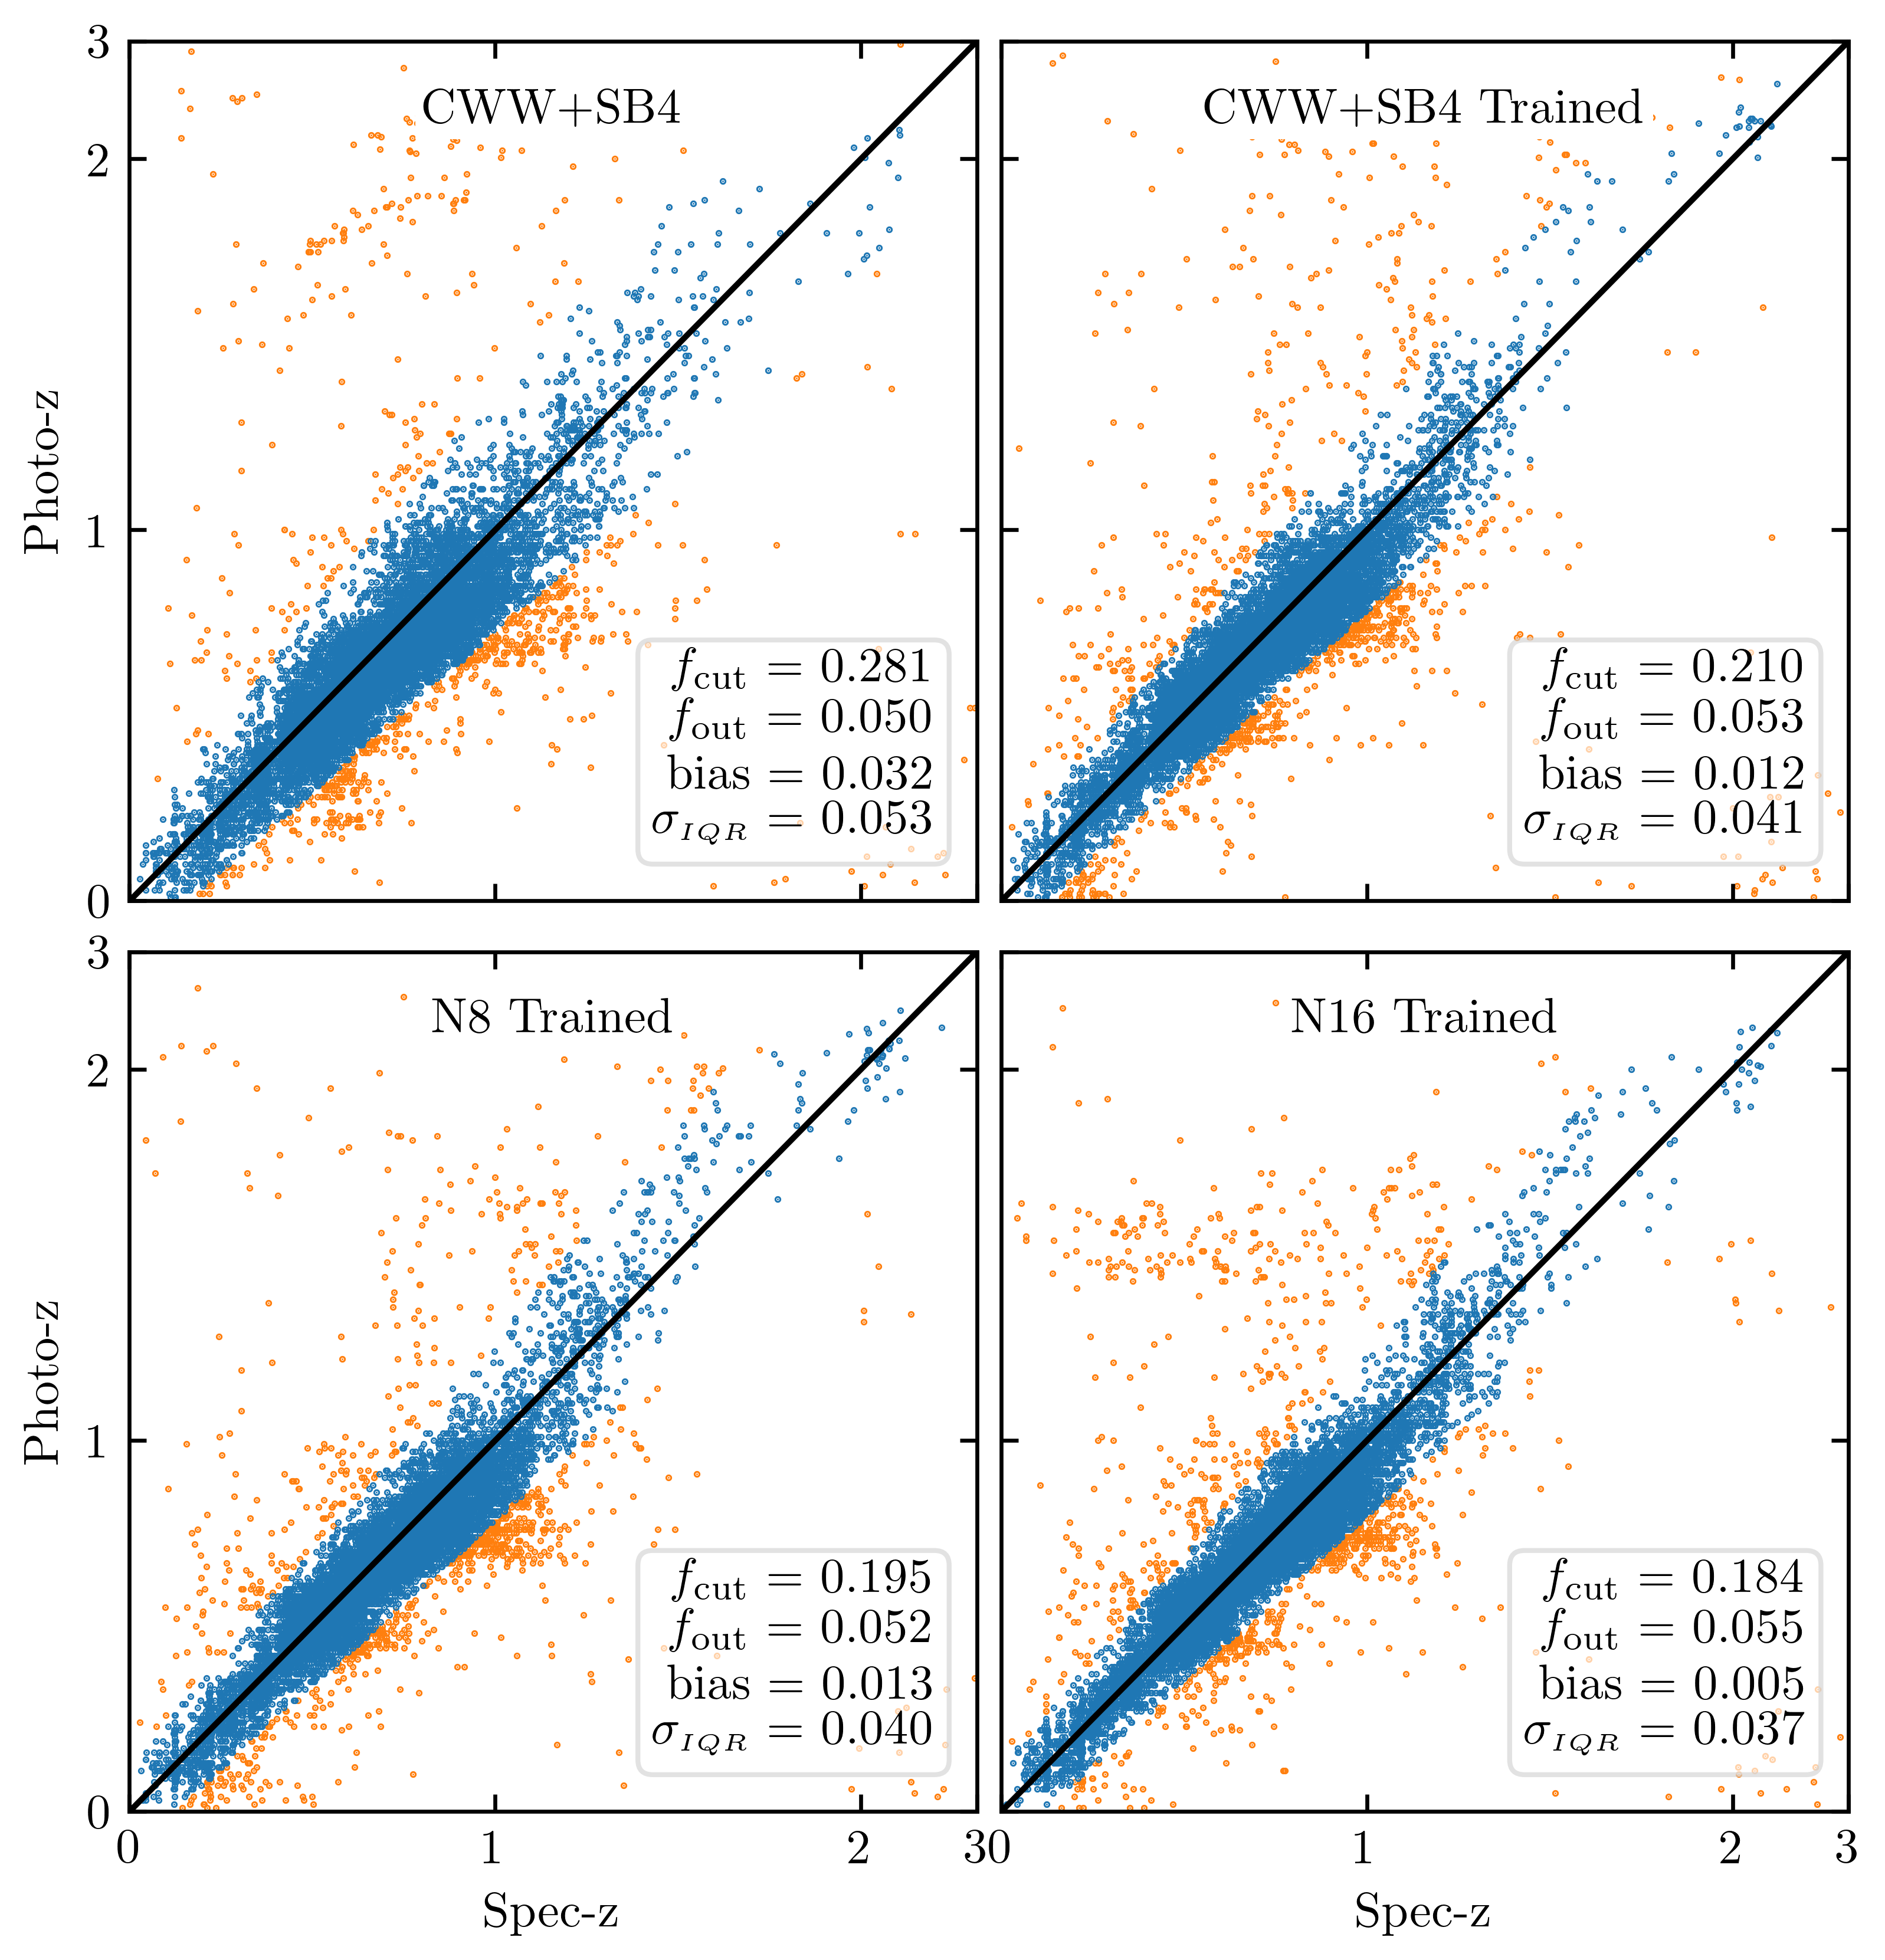
\includegraphics{photoz_results.png}
    \caption{Results of photo-z estimation with \bpz, using the four different templates sets. Photo-z estimates are displayed as points: inliers are blue and outliers are orange. The black line represents perfect estimation (i.e. photo-z = spec-z). The statistics printed in each panel are for the entire data set.}
    \label{fig:photoz_results}
\end{figure*}

The photo-z results can be seen in Figure \ref{fig:photoz_results}.
The photo-z estimates that passed the cuts on \texttt{ODDS} and $\chi_\text{mod}^2$ are displayed as points: the inliers in blue, the outliers in orange.
The values of the photo-z statistics for each template set are printed in each panel.
For all four template sets, the photo-z estimation is reasonably accurate for spec-z's $z < 1.5$.
For higher redshifts, there appears to be a systematic bias towards higher photo-z's.
Reduced photo-z accuracy is generally expected for spec-z's greater than 1.5, as the Balmer break leaves most band sets at around $z=1.4$ and the Lyman break does not enter most band sets until $z=2.5$.

For the CWW+SB4 templates, the training algorithm decreased the fraction of photo-z's cut by 25\%, the bias by 63\%, and the scatter by 23\%, but did not improve the outlier fraction.
We were able to achieve similar photo-z results using the trained N8 and N16 template sets, demonstrating that our training algorithm can be used to generate photo-z templates without any a priori information about galaxy spectra.
Compared to the CWW+SB4 templates, N8 templates decreased $f_\text{cut}$ by 31\%, bias by 59\%, and scatter by 25\%.
The N16 templates decreased $f_\text{cut}$ by 35\%, bias by 84\%, and scatter by 30\%.
However, both sets have slightly increased outlier fractions.

Comparing the results for the N8 and N16 template sets indicate that increasing the number of templates can reduce the fraction cut, and the bias and scatter of the photo-z estimates.
To further investigate this relationship, we calculate the photo-z statistics for a range of template numbers, the results of which are in Figure \ref{fig:Ntemplates}.
We find that increasing the number of templates decreases the fraction cut and the bias, as well as slightly decreasing the scatter.
The trend for outlier fraction is less clear.

The N20 set has $f_\text{cut} = 0.188$ (a 33\% decrease compared to CWW+SB4), $f_\text{out} = 0.040$ (a 20\% decrease), bias = 0.003 (a 91\% decrease), and scatter = 0.039 (a 26\% decrease).

\begin{figure*}
    \centering
    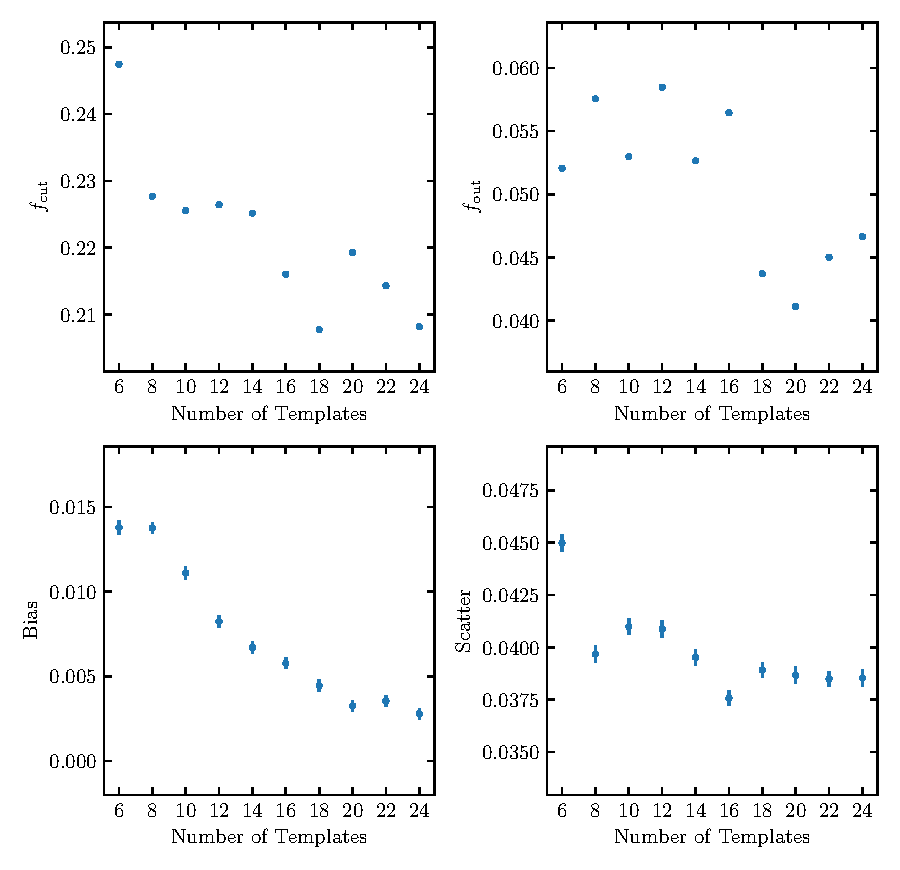
\includegraphics{figures/Ntemplates.pdf}
    \caption{Photo-z statistics as a function of template number. Statistics are for the full redshift range.}
    \label{fig:Ntemplates}
\end{figure*}

The value of the metrics as a function of photo-z can be seen in Figure \ref{fig:photoz_binned}.
In addition to the template sets plotted above, we add the N20 set.
For comparison, plotted in gray are the LSST science requirements for the metrics as listed in the LSST Science Requirement Document (SRD; \citealt{Ivezic2018}).
The SRD lists the following minimum requirements to enable the envisioned LSST cosmological studies: root-mean-square error $< 0.02(1+z_\text{phot})$; $f_\text{out} < 10\%$; average bias $<0.003(1+z_\text{phot})$.
The SRD lists these requirements for an $i<25$, magnitude-limited sample of four billion galaxies from $0.3 < z < 3.0$.
For comparison, our test set consists of 20,496 galaxies with $i < 25.7$, in the range $z < 3.6$, including 19,391 galaxies with $i < 25$, in the range $0.3 < z < 3.0$.
In Figure \ref{fig:photoz_binned}, you can see that for redshifts $0.3 < z < 1.2$ we are able to achieve an appropriate outlier fraction, and that our training algorithm makes great progress on the bias, almost reaching the threshold required for LSST.
We also make modest progress on the scatter, but reduction by another factor of two is still required.
Beyond redshift $z=1.2$, all of our metrics far exceed the LSST science requirements.

\begin{figure*}
    \centering
    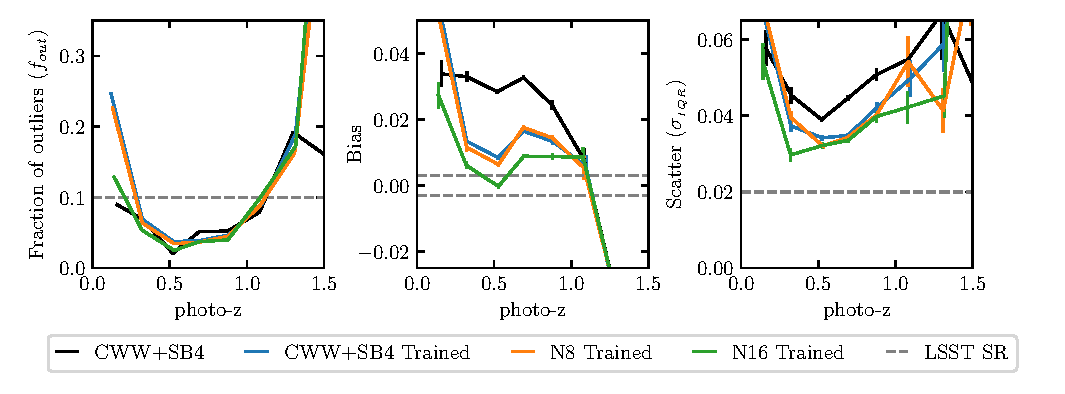
\includegraphics{figures/photoz_binned_metrics.pdf}
    \caption{Photo-z metrics for the various template sets as a function of redshift bin. LSST science requirements are shown as dashed gray lines.}
    \label{fig:photoz_binned}
\end{figure*}

\section{Discussion}
    
\label{sect:discussion}

In Section \ref{sect:template_training}, we demonstrated that our training algorithm could learn galaxy SED templates from photometry at a high resolution relative to the filters used to make the observations.
We are able to well learn a set of templates over twice the size of the standard CWW+SB4, showing a smooth progression of galaxy colors from red to blue.
The spectra contain relatively high resolution spectral features, and post-processing can further reconstruct emission and absorption lines.
However, our method has a number of limitations.

The success of our algorithm relies on the ability to generate a naive set of templates as a starting point that will reliably divide the photometry by the spectral type of the galaxy. 
This is relatively easy to accomplish for fewer than 20 templates, as was demonstrated by our simple photometry matching procedure and the log-normal templates we used.
This is a strength of the algorithm, as it is relatively robust to the starting templates, however if you wish to derive more than 20 templates from the photometry, more care must be taken in the division of the photometry set.
Attempts at reconstructing more than 20 templates usually result in some templates not having sufficient photometry across the entire wavelength range of interest.
In addition, the inherently discretized way in which we divide the photometry set stands in the way of generating a truly continuous set of SED templates.
For a more continuous set of templates, it would be advantageous to devise a method to assemble more continuous, non-exclusive photometry sets.
For example, one might imagine taking two ``adjacent'' photometry sets, and assembling a photometry set ``between'' them by taking the bluer half on one set together with the redder half of the other.

Our data consists only of broadband photometry, however our algorithm would work equally well with narrow bands as well.
Combining broadband and narrow band photometry would expand the data set and further constrain the templates.
In particular, the addition of narrowband photometry should increase the resolution of spectral features recovered, and may allow one to resolve features such as the H$\gamma$ and H$\delta$ emission lines that we had to treat as a single feature.
One could also include bands from a wider range of wavelengths to increase the wavelength range over which the templates are constrained.
We attempted to include fluxes from the $K$-bands included with the zCOSMOS and VIPERS catalogs to learn the high-wavelength tails of the templates, but there appeared to be systematic normalization issues we did not resolve.
There is evidence that the inclusion of near-infrared and near-ultraviolet photometry in photo-z estimation can reduce outliers and scatter by up to 50\% each \citep{Graham2020}.

In addition, for the results presented here, we used only galaxy fluxes with SNR greater than 20.
One can use galaxies with lower SNR if outlier fluxes are removed from the photometry sets before training (we had success using an Isolation Forest; \citealt{Ting2008,Liu2012}).
However, lowering the SNR of the photometry generally reduces the resolution of the structure you can reconstruct.
For even better results, it would be good to check that all of the photometry is aperture corrected, properly normalized, etc.

The training algorithm itself could be made more sophisticated by restoring the wavelength dependence of the hyperparameter $\Delta_k$.
We also hope to move beyond an iterative regression approach into deep learning, perhaps using Generative Adversarial Networks (GANs; \citealt{Goodfellow2014}).

We found in Section \ref{sect:photoz_results} that our training algorithm can improve the bias and scatter of photo-z estimates.
We found that increasing the number of templates enhances these improvements, with the best results for 20 templates.
As mentioned above, with our current method for generating photometry sets, we struggle to reliably reconstruct more than 20 templates, so whether these benefits continue to decrease with template number is unknown.

We can compare our method for generating more SED templates with \bpz's method of linearly interpolating between templates.
N8 with \texttt{INTERP=2} generates 22 total templates.
Table \ref{tab:interp_comparison} compares the photo-z results using these templates with the results using 22 templates learned from the photometry with \texttt{INTERP=0}.
It is clear that, as far as $f_\text{out}$ and bias, our method for generating extra templates is superior to the linear interpolation used by \bpz. 

\begin{table}[h]
    \caption{Comparison of photo-z results for the N8 templates with \texttt{INTERP=0,2} and the N22 templates with \texttt{INTERP=0}. Statistics quoted are for the full redshift range.}
    \label{tab:interp_comparison}
    \centering
    \begin{tabular}{c c c c c c c}
        \hline \hline
        & \texttt{INTERP} & Total N & $f_\text{cut}$ & $f_\text{out}$ & Bias & Scatter \\
        \hline

        N8  & 0 &  8 & 0.228 & 0.058 & 0.014 & 0.040 \\
        N8  & 2 & 22 & 0.209 & 0.060 & 0.012 & 0.037 \\
        N22 & 0 & 22 & 0.214 & 0.045 & 0.004 & 0.039 \\

        \hline
    \end{tabular}
\end{table}

The photo-z estimation with our learned template sets outperforms the results of the standard CWW+SB4 templates, however, more work needs to be done to reach the requirements set for LSST, especially for redshifts $z>1$.
Templates can be trained for LSST science using the substantial overlap of LSST photometry with the eBoss \citep{Dawson2016} and Dark Energy Spectroscopic Instrument (DESI; \citealt{DESICollaboration2016}) surveys which will provide hundreds of thousands of spec-z's for LSST photo-z training and calibration \citep{Schmidt2014,Newman2015}.

Our training method can be extended to other domains where you can take a large set of incomplete data, segment that data into classes, and treat the set of unique observations in each class as an ensemble of observations of some class archetype, and thereby reconstruct more complete information.
We plan to adapt the method to reconstruct supernova lightcurves from supernova photometry.
This extends the spectra we have been reconstructing into the time domain, and amounts to iteratively learning the shape of a surface rather than a one dimensional distribution.


%N8 interp 0- 
%fcut=0.234
%fout=0.059, 
%bias=0.0138 0.0003
%scatter=0.0397 0.0004
%N8 interp 2- 
%fcut=0.209
%fout=0.060, 
%bias=0.0123 0.0003
%scatter=0.0370 0.0004
%N22 interp 0- 
%fcut=0.214
%fout=0.045, 
%bias=0.0035 0.0003
%scatter=0.0385 0.0004
    
\section{Conclusions}
    
\label{sect:conclusion}

We have shown that galaxy SED templates can be learned directly from a data set of broadband photometry.
Large sets of photometry at various redshifts can be leveraged to reconstruct high resolution features, such as the H$\alpha$, H$\beta$, H$\gamma$, H$\delta$, OII, and OIII emission lines, as well as Na and Mg absorption lines.
Simple post processing can further reconstruct these features and provide information such as line ratios and equivalent width.
The number of templates learned is variable and can be increased to more continuously sample the space of galaxy spectra and to improve photo-z results.
However, our current method of generating photometry sets for training is inherently discrete, and a more continuous method needs to be developed to increase the continuity of the templates.

We used our templates to estimate photo-z's for a test set of galaxies using \bpz.
We found that training the standard set of templates that comes with \bpz\ decreases the bias of the photo-z's by 61\% and the scatter by 21\%, but does not improve the outlier fraction.
Our own trained naive templates yielded better results.
We learned a set of 20 templates from the data that reduced the fraction of outliers by 28\%, the bias by 91\%, and the scatter by 25\%.
The improvements in bias are almost sufficient to meet the requirements set for LSST, but another reduction by a factor of two is needed for the scatter.

The templates derived with our training algorithm demonstrate that accurate galaxy spectra can be learned from broadband photometry.
Our SED's could potentially be used for applications other than photo-z's, and our learning algorithm can be extended to other applications, such as learning supernova lightcurves from photometry.

Our derived templates and the code used to produce these results are publicly available in a dedicated Github repository: \url{https://github.com/dirac-institute/photoz_template_learning}.

\acknowledgments

The authors would like to thank Bryce Kalmbach for providing advice in early stages of this work, Sam Schmidt for his help with \bpz\, and Melissa Graham for her code to calculate photo-z statistics.
This work was supported by the U.S. Department of Energy, Office of Science, under Award Number \note{NUMBER}.

This research is based on observations made with ESO Telescopes at the La Silla or Paranal Observatories under programme ID(s) 175.A-0839(B), 175.A-0839(D), 175.A-0839(I), 175.A-0839(J), 175.A-0839(H), 175.A-0839(F).
This research is also based on observations obtained with MegaPrime/MegaCam, a joint project of CFHT and CEA/DAPNIA, at the Canada-France-Hawaii Telescope (CFHT) which is operated by the National Research Council (NRC) of Canada, the Institut National des Science de l'Univers of the Centre National de la Recherche Scientifique (CNRS) of France, and the University of Hawaii.
This research is also based in part on data products produced at Terapix available at the Canadian Astronomy Data Centre as part of the Canada-France-Hawaii Telescope Legacy Survey, a collaborative project of NRC and CNRS.
We use data from the VIMOS VLT Deep Survey, obtained from the VVDS database operated by Cesam, Laboratoire d'Astrophysique de Marseille, France
We also use data from the VIMOS Public Extragalactic Redshift Survey (VIPERS).
VIPERS has been performed using the ESO Very Large Telescope, under the "Large Programme" 182.A-0886. 
The participating institutions and funding agencies are listed at \url{http://vipers.inaf.it}
This research has also made use of the SVO Filter Profile Service (\url{http://svo2.cab.inta-csic.es/theory/fps/}) supported from the Spanish MINECO through grant AYA2017-84089.

\software{Astropy \citep{AstropyCollaboration2013}, BPZ \citep{Benitez2000a}, Jupyter \citep{Kluyver2016}, Matplotlib \citep{Hunter2007}, Numpy \citep{VanDerWalt2011}, Scikit-learn \citep{Pedregosa2011}, Scipy \citep{Virtanen2020}.}
    


\bibliography{references.bib}{}
\bibliographystyle{aasjournal}

\end{document}
